% Generated by Sphinx.
\def\sphinxdocclass{report}
\documentclass[a5paper,10pt,spanish]{sphinxmanual}
\usepackage[utf8]{inputenc}
\DeclareUnicodeCharacter{00A0}{\nobreakspace}
\usepackage{cmap}
\usepackage[T1]{fontenc}
\usepackage{babel}
\usepackage{times}
\usepackage[Sonny]{fncychap}
\usepackage{longtable}
\usepackage{sphinx}
\usepackage{multirow}


\title{Programación PHP}
\date{14 de April de 2014}
\release{}
\author{Armando Arce}
\newcommand{\sphinxlogo}{}
\renewcommand{\releasename}{Publicación}
\makeindex

\makeatletter
\def\PYG@reset{\let\PYG@it=\relax \let\PYG@bf=\relax%
    \let\PYG@ul=\relax \let\PYG@tc=\relax%
    \let\PYG@bc=\relax \let\PYG@ff=\relax}
\def\PYG@tok#1{\csname PYG@tok@#1\endcsname}
\def\PYG@toks#1+{\ifx\relax#1\empty\else%
    \PYG@tok{#1}\expandafter\PYG@toks\fi}
\def\PYG@do#1{\PYG@bc{\PYG@tc{\PYG@ul{%
    \PYG@it{\PYG@bf{\PYG@ff{#1}}}}}}}
\def\PYG#1#2{\PYG@reset\PYG@toks#1+\relax+\PYG@do{#2}}

\expandafter\def\csname PYG@tok@gd\endcsname{\def\PYG@tc##1{\textcolor[rgb]{0.63,0.00,0.00}{##1}}}
\expandafter\def\csname PYG@tok@gu\endcsname{\let\PYG@bf=\textbf\def\PYG@tc##1{\textcolor[rgb]{0.50,0.00,0.50}{##1}}}
\expandafter\def\csname PYG@tok@gt\endcsname{\def\PYG@tc##1{\textcolor[rgb]{0.00,0.27,0.87}{##1}}}
\expandafter\def\csname PYG@tok@gs\endcsname{\let\PYG@bf=\textbf}
\expandafter\def\csname PYG@tok@gr\endcsname{\def\PYG@tc##1{\textcolor[rgb]{1.00,0.00,0.00}{##1}}}
\expandafter\def\csname PYG@tok@cm\endcsname{\let\PYG@it=\textit\def\PYG@tc##1{\textcolor[rgb]{0.25,0.50,0.56}{##1}}}
\expandafter\def\csname PYG@tok@vg\endcsname{\def\PYG@tc##1{\textcolor[rgb]{0.73,0.38,0.84}{##1}}}
\expandafter\def\csname PYG@tok@m\endcsname{\def\PYG@tc##1{\textcolor[rgb]{0.13,0.50,0.31}{##1}}}
\expandafter\def\csname PYG@tok@mh\endcsname{\def\PYG@tc##1{\textcolor[rgb]{0.13,0.50,0.31}{##1}}}
\expandafter\def\csname PYG@tok@cs\endcsname{\def\PYG@tc##1{\textcolor[rgb]{0.25,0.50,0.56}{##1}}\def\PYG@bc##1{\setlength{\fboxsep}{0pt}\colorbox[rgb]{1.00,0.94,0.94}{\strut ##1}}}
\expandafter\def\csname PYG@tok@ge\endcsname{\let\PYG@it=\textit}
\expandafter\def\csname PYG@tok@vc\endcsname{\def\PYG@tc##1{\textcolor[rgb]{0.73,0.38,0.84}{##1}}}
\expandafter\def\csname PYG@tok@il\endcsname{\def\PYG@tc##1{\textcolor[rgb]{0.13,0.50,0.31}{##1}}}
\expandafter\def\csname PYG@tok@go\endcsname{\def\PYG@tc##1{\textcolor[rgb]{0.20,0.20,0.20}{##1}}}
\expandafter\def\csname PYG@tok@cp\endcsname{\def\PYG@tc##1{\textcolor[rgb]{0.00,0.44,0.13}{##1}}}
\expandafter\def\csname PYG@tok@gi\endcsname{\def\PYG@tc##1{\textcolor[rgb]{0.00,0.63,0.00}{##1}}}
\expandafter\def\csname PYG@tok@gh\endcsname{\let\PYG@bf=\textbf\def\PYG@tc##1{\textcolor[rgb]{0.00,0.00,0.50}{##1}}}
\expandafter\def\csname PYG@tok@ni\endcsname{\let\PYG@bf=\textbf\def\PYG@tc##1{\textcolor[rgb]{0.84,0.33,0.22}{##1}}}
\expandafter\def\csname PYG@tok@nl\endcsname{\let\PYG@bf=\textbf\def\PYG@tc##1{\textcolor[rgb]{0.00,0.13,0.44}{##1}}}
\expandafter\def\csname PYG@tok@nn\endcsname{\let\PYG@bf=\textbf\def\PYG@tc##1{\textcolor[rgb]{0.05,0.52,0.71}{##1}}}
\expandafter\def\csname PYG@tok@no\endcsname{\def\PYG@tc##1{\textcolor[rgb]{0.38,0.68,0.84}{##1}}}
\expandafter\def\csname PYG@tok@na\endcsname{\def\PYG@tc##1{\textcolor[rgb]{0.25,0.44,0.63}{##1}}}
\expandafter\def\csname PYG@tok@nb\endcsname{\def\PYG@tc##1{\textcolor[rgb]{0.00,0.44,0.13}{##1}}}
\expandafter\def\csname PYG@tok@nc\endcsname{\let\PYG@bf=\textbf\def\PYG@tc##1{\textcolor[rgb]{0.05,0.52,0.71}{##1}}}
\expandafter\def\csname PYG@tok@nd\endcsname{\let\PYG@bf=\textbf\def\PYG@tc##1{\textcolor[rgb]{0.33,0.33,0.33}{##1}}}
\expandafter\def\csname PYG@tok@ne\endcsname{\def\PYG@tc##1{\textcolor[rgb]{0.00,0.44,0.13}{##1}}}
\expandafter\def\csname PYG@tok@nf\endcsname{\def\PYG@tc##1{\textcolor[rgb]{0.02,0.16,0.49}{##1}}}
\expandafter\def\csname PYG@tok@si\endcsname{\let\PYG@it=\textit\def\PYG@tc##1{\textcolor[rgb]{0.44,0.63,0.82}{##1}}}
\expandafter\def\csname PYG@tok@s2\endcsname{\def\PYG@tc##1{\textcolor[rgb]{0.25,0.44,0.63}{##1}}}
\expandafter\def\csname PYG@tok@vi\endcsname{\def\PYG@tc##1{\textcolor[rgb]{0.73,0.38,0.84}{##1}}}
\expandafter\def\csname PYG@tok@nt\endcsname{\let\PYG@bf=\textbf\def\PYG@tc##1{\textcolor[rgb]{0.02,0.16,0.45}{##1}}}
\expandafter\def\csname PYG@tok@nv\endcsname{\def\PYG@tc##1{\textcolor[rgb]{0.73,0.38,0.84}{##1}}}
\expandafter\def\csname PYG@tok@s1\endcsname{\def\PYG@tc##1{\textcolor[rgb]{0.25,0.44,0.63}{##1}}}
\expandafter\def\csname PYG@tok@gp\endcsname{\let\PYG@bf=\textbf\def\PYG@tc##1{\textcolor[rgb]{0.78,0.36,0.04}{##1}}}
\expandafter\def\csname PYG@tok@sh\endcsname{\def\PYG@tc##1{\textcolor[rgb]{0.25,0.44,0.63}{##1}}}
\expandafter\def\csname PYG@tok@ow\endcsname{\let\PYG@bf=\textbf\def\PYG@tc##1{\textcolor[rgb]{0.00,0.44,0.13}{##1}}}
\expandafter\def\csname PYG@tok@sx\endcsname{\def\PYG@tc##1{\textcolor[rgb]{0.78,0.36,0.04}{##1}}}
\expandafter\def\csname PYG@tok@bp\endcsname{\def\PYG@tc##1{\textcolor[rgb]{0.00,0.44,0.13}{##1}}}
\expandafter\def\csname PYG@tok@c1\endcsname{\let\PYG@it=\textit\def\PYG@tc##1{\textcolor[rgb]{0.25,0.50,0.56}{##1}}}
\expandafter\def\csname PYG@tok@kc\endcsname{\let\PYG@bf=\textbf\def\PYG@tc##1{\textcolor[rgb]{0.00,0.44,0.13}{##1}}}
\expandafter\def\csname PYG@tok@c\endcsname{\let\PYG@it=\textit\def\PYG@tc##1{\textcolor[rgb]{0.25,0.50,0.56}{##1}}}
\expandafter\def\csname PYG@tok@mf\endcsname{\def\PYG@tc##1{\textcolor[rgb]{0.13,0.50,0.31}{##1}}}
\expandafter\def\csname PYG@tok@err\endcsname{\def\PYG@bc##1{\setlength{\fboxsep}{0pt}\fcolorbox[rgb]{1.00,0.00,0.00}{1,1,1}{\strut ##1}}}
\expandafter\def\csname PYG@tok@kd\endcsname{\let\PYG@bf=\textbf\def\PYG@tc##1{\textcolor[rgb]{0.00,0.44,0.13}{##1}}}
\expandafter\def\csname PYG@tok@ss\endcsname{\def\PYG@tc##1{\textcolor[rgb]{0.32,0.47,0.09}{##1}}}
\expandafter\def\csname PYG@tok@sr\endcsname{\def\PYG@tc##1{\textcolor[rgb]{0.14,0.33,0.53}{##1}}}
\expandafter\def\csname PYG@tok@mo\endcsname{\def\PYG@tc##1{\textcolor[rgb]{0.13,0.50,0.31}{##1}}}
\expandafter\def\csname PYG@tok@mi\endcsname{\def\PYG@tc##1{\textcolor[rgb]{0.13,0.50,0.31}{##1}}}
\expandafter\def\csname PYG@tok@kn\endcsname{\let\PYG@bf=\textbf\def\PYG@tc##1{\textcolor[rgb]{0.00,0.44,0.13}{##1}}}
\expandafter\def\csname PYG@tok@o\endcsname{\def\PYG@tc##1{\textcolor[rgb]{0.40,0.40,0.40}{##1}}}
\expandafter\def\csname PYG@tok@kr\endcsname{\let\PYG@bf=\textbf\def\PYG@tc##1{\textcolor[rgb]{0.00,0.44,0.13}{##1}}}
\expandafter\def\csname PYG@tok@s\endcsname{\def\PYG@tc##1{\textcolor[rgb]{0.25,0.44,0.63}{##1}}}
\expandafter\def\csname PYG@tok@kp\endcsname{\def\PYG@tc##1{\textcolor[rgb]{0.00,0.44,0.13}{##1}}}
\expandafter\def\csname PYG@tok@w\endcsname{\def\PYG@tc##1{\textcolor[rgb]{0.73,0.73,0.73}{##1}}}
\expandafter\def\csname PYG@tok@kt\endcsname{\def\PYG@tc##1{\textcolor[rgb]{0.56,0.13,0.00}{##1}}}
\expandafter\def\csname PYG@tok@sc\endcsname{\def\PYG@tc##1{\textcolor[rgb]{0.25,0.44,0.63}{##1}}}
\expandafter\def\csname PYG@tok@sb\endcsname{\def\PYG@tc##1{\textcolor[rgb]{0.25,0.44,0.63}{##1}}}
\expandafter\def\csname PYG@tok@k\endcsname{\let\PYG@bf=\textbf\def\PYG@tc##1{\textcolor[rgb]{0.00,0.44,0.13}{##1}}}
\expandafter\def\csname PYG@tok@se\endcsname{\let\PYG@bf=\textbf\def\PYG@tc##1{\textcolor[rgb]{0.25,0.44,0.63}{##1}}}
\expandafter\def\csname PYG@tok@sd\endcsname{\let\PYG@it=\textit\def\PYG@tc##1{\textcolor[rgb]{0.25,0.44,0.63}{##1}}}

\def\PYGZbs{\char`\\}
\def\PYGZus{\char`\_}
\def\PYGZob{\char`\{}
\def\PYGZcb{\char`\}}
\def\PYGZca{\char`\^}
\def\PYGZam{\char`\&}
\def\PYGZlt{\char`\<}
\def\PYGZgt{\char`\>}
\def\PYGZsh{\char`\#}
\def\PYGZpc{\char`\%}
\def\PYGZdl{\char`\$}
\def\PYGZhy{\char`\-}
\def\PYGZsq{\char`\'}
\def\PYGZdq{\char`\"}
\def\PYGZti{\char`\~}
% for compatibility with earlier versions
\def\PYGZat{@}
\def\PYGZlb{[}
\def\PYGZrb{]}
\makeatother

\begin{document}
\shorthandoff{"}
\maketitle
\tableofcontents
\phantomsection\label{index::doc}


El objetivo de este sitio es presentar una serie de tutoriales básicos sobre el desarrollo de aplicaciones web utilizando el lenguaje PHP.

Los tutoriales disponibles hasta el momento son los siguientes:


\chapter{Contenidos}
\label{index:contenidos}\label{index:programacion-php}

\section{Introducción a PHP}
\label{Tutorial1_Conceptos.md:introduccion-a-php}\label{Tutorial1_Conceptos.md::doc}
PHP es un lenguaje diseñado para crear contenido HTML. PHP puede ser
ejecutado de tres formas: en un servidor web, a través de la línea de
comandos, o mediante un cliente GUI.

El lenguaje puede ejecutarse en prácticamente todos los sistemas
operativos actuales y en múltiples servidores web. Este también soporta
una amplia variedad de bases de datos y cuenta con múltiples librerías
para ejecutar procesos comunes.

Una página PHP generalmente consiste de una página HTML con comandos PHP
incrustados en ella. El servidor web procesa los comandos PHP y envía la
salida al visualizador (browser). Un ejemplo de una página PHP sencilla
sería la siguiente:

Una página PHP generalmente consiste de una página HTML con comandos PHP
incrustados en ella. El servidor web procesa los comandos PHP y envía la
salida al visualizador (browser). Un ejemplo de una página PHP sencilla
sería la siguiente:

\begin{Verbatim}[commandchars=\\\{\}]
\PYGZlt{}html\PYGZgt{}
  \PYGZlt{}head\PYGZgt{} \PYGZlt{}title\PYGZgt{}Hello, world\PYGZlt{}/title\PYGZgt{} \PYGZlt{}/head\PYGZgt{}
  \PYGZlt{}body\PYGZgt{}
    \PYGZlt{}?php echo \PYGZdq{}Hello, world!\PYGZdq{}; ?\PYGZgt{}
  \PYGZlt{}/body\PYGZgt{}
\PYGZlt{}/html\PYGZgt{}
\end{Verbatim}

El comando \emph{echo} de PHP produce la salida que se inserta en la página
HTML. Note que el código PHP se escribe dentro de los delimitadores
\emph{\textless{}?php} y \emph{?\textgreater{}}.

Las instrucciones se separan con \emph{`;'}, en el caso de ser la última
instrucción no es necesario el punto y coma.

Los comentarios en PHP pueden ser:
\begin{itemize}
\item {} 
Como en C o C++, /*...*/ ó //

\item {} 
Otro tipo de comentario de una línea es \#, que comentará la línea en
la que aparezca pero sólo hasta el tag \emph{?\textgreater{}} que cierra el código php.

\end{itemize}


\subsection{Tipos de Datos}
\label{Tutorial1_Conceptos.md:tipos-de-datos}
Los tipos de cada variable en PHP no están tan claros como en C. El
intérprete asigna el tipo de una variable según el uso que se esté
haciendo de ella. Para asignar un tipo fijo a una variable se utiliza la
función settype(). Los tipos
son:
\begin{itemize}
\item {} 
Enteros

\item {} 
Flotantes

\item {} 
String

\item {} 
arreglos

\item {} 
Objetos

\item {} 
Variables variables

\end{itemize}

El siguiente ejemplo muestra la utilización de los tipos de datos
enteros y flotantes. Los otros tipos de datos se describen más adelante.

\begin{Verbatim}[commandchars=\\\{\}]
\PYGZlt{}html\PYGZgt{}
\PYGZlt{}head\PYGZgt{} \PYGZlt{}title\PYGZgt{}Ejemplo 2 \PYGZlt{}/title\PYGZgt{}\PYGZlt{}/head\PYGZgt{}
\PYGZlt{}body\PYGZgt{}
 \PYGZlt{}h1\PYGZgt{} Ejemplo de PHP \PYGZlt{}/h1\PYGZgt{}

\PYGZlt{}?php

 \PYGZsh{}Enteros
 \PYGZdl{}a = 1234; \PYGZsh{} número decimal
 \PYGZdl{}a = \PYGZhy{}123; \PYGZsh{} un número negativo
 \PYGZdl{}a = 0123; \PYGZsh{} número octal (equivalente al 83 decimal)
 \PYGZdl{}a = 0x12; /* número hexadecimal (equivalente al 18 decimal) */

 //Flotantes o reales
 \PYGZdl{}b = 1.234; \PYGZdl{}b = 1.2e3;

 //Escribimos algo
 print \PYGZdq{}\PYGZbs{}n La a= \PYGZdl{}a y la b= \PYGZdl{}b \PYGZlt{}br\PYGZgt{}\PYGZbs{}n\PYGZdq{};
?\PYGZgt{}

\PYGZlt{}/body\PYGZgt{}
\PYGZlt{}/html\PYGZgt{}
\end{Verbatim}


\subsubsection{Hileras de texto}
\label{Tutorial1_Conceptos.md:hileras-de-texto}
Las hileras de texto pueden estar delimitadas por \emph{'' o `}. Si la hilera
de texto está delimitada por comillas dobles, cualquier variable
incluida dentro de ella será sustituida por su valor (ver y ejecutar el
ejemplo anterior). Para especificar el carácter \emph{``} se escapará con el
carácter backslash( \textbackslash{} ).

Las operaciones con hileras de texto son exactamente igual que en PERL.
Por ejemplo, con strlen se ve
el tamaño de una hilera de texto y con el punto ( . ) se concatenan
hileras de texto.

\begin{Verbatim}[commandchars=\\\{\}]
\PYGZlt{}html\PYGZgt{}
\PYGZlt{}head\PYGZgt{} \PYGZlt{}title\PYGZgt{}Ejemplo 3 \PYGZlt{}/title\PYGZgt{}\PYGZlt{}/head\PYGZgt{}
\PYGZlt{}body\PYGZgt{}
 \PYGZlt{}h1\PYGZgt{} Ejemplo de PHP \PYGZlt{}/h1\PYGZgt{}

\PYGZlt{}?php
 /* Asignando una hilera de texto. */
 \PYGZdl{}str = \PYGZdq{}Esto es una hilera de texto\PYGZdq{};

 /* Añadiendo a la hilera de texto. */
 \PYGZdl{}str = \PYGZdl{}str . \PYGZdq{} con algo más de texto\PYGZdq{};

 /* Otra forma de añadir, incluye un carácter de nueva línea  */
 \PYGZdl{}str .= \PYGZdq{} Y un carácter de nueva línea al final.\PYGZbs{}n\PYGZdq{};
 print \PYGZdq{}\PYGZdl{}str \PYGZlt{}br\PYGZgt{}\PYGZbs{}n\PYGZdq{};

 /* Esta hilera de texto terminará siendo \PYGZsq{}\PYGZlt{}p\PYGZgt{}Número: 9\PYGZlt{}/p\PYGZgt{}\PYGZsq{} */
 \PYGZdl{}num = 9;
 \PYGZdl{}str = \PYGZdq{}\PYGZlt{}p\PYGZgt{}Número: \PYGZdl{}num\PYGZlt{}/p\PYGZgt{}\PYGZdq{};
 print \PYGZdq{}\PYGZdl{}str \PYGZlt{}br\PYGZgt{}\PYGZbs{}n\PYGZdq{};

 /* Esta será \PYGZsq{}\PYGZlt{}p\PYGZgt{}Número: \PYGZdl{}num\PYGZlt{}/p\PYGZgt{}\PYGZsq{} */
 \PYGZdl{}num = 9;
 \PYGZdl{}str = \PYGZsq{}\PYGZlt{}p\PYGZgt{}Número: \PYGZdl{}num\PYGZlt{}/p\PYGZgt{}\PYGZsq{};
 print \PYGZdq{}\PYGZdl{}str \PYGZlt{}br\PYGZgt{}\PYGZbs{}n\PYGZdq{};

 /* Obtener el primer carácter de una hilera de texto  como una vector*/
 \PYGZdl{}str = \PYGZsq{}Esto es una prueba.\PYGZsq{};
 \PYGZdl{}first = \PYGZdl{}str[0];
 print \PYGZdq{}\PYGZdl{}str 0\PYGZhy{}\PYGZgt{}\PYGZdl{}first \PYGZlt{}br\PYGZgt{}\PYGZbs{}n\PYGZdq{};

 /* Obtener el último carácter de una hilera de texto. */
 \PYGZdl{}str = \PYGZsq{}Esto es aún una prueba.\PYGZsq{};
 \PYGZdl{}last = \PYGZdl{}str[strlen(\PYGZdl{}str)\PYGZhy{}1];
 print \PYGZdq{}\PYGZdl{}str last\PYGZhy{}\PYGZgt{}\PYGZdl{}last \PYGZlt{}br\PYGZgt{}\PYGZbs{}n\PYGZdq{};
 ?\PYGZgt{}

\PYGZlt{}/body\PYGZgt{}
\PYGZlt{}/html\PYGZgt{}
\end{Verbatim}

Para hacer conversión de hileras de texto a otros tipos de datos hay que
tener en cuenta una hilera de texto se evalúa como un valor numérico, el
valor resultante y el tipo se determinan como sigue. La hilera de texto
se evaluará como un doble si contiene cualquiera de los caracteres `.',
`e', o `E'. En caso contrario, se evaluará como un entero. El valor
viene dado por la porción inicial de la hilera de texto. Si la hilera de
texto comienza con datos de valor numérico, este será el valor usado. En
caso contrario, el valor será 0 (cero). Cuando la primera expresión es
una hilera de texto, el tipo de la variable dependerá de la segunda
expresión.

\begin{Verbatim}[commandchars=\\\{\}]
\PYGZlt{}html\PYGZgt{}
\PYGZlt{}head\PYGZgt{} \PYGZlt{}title\PYGZgt{}Ejemplo 4\PYGZlt{}/title\PYGZgt{}\PYGZlt{}/head\PYGZgt{}
\PYGZlt{}body\PYGZgt{}
 \PYGZlt{}h1\PYGZgt{} Ejemplo de PHP \PYGZlt{}/h1\PYGZgt{}

\PYGZlt{}?php

 \PYGZdl{}foo = 1 + \PYGZdq{}10.5\PYGZdq{};              // \PYGZdl{}foo es doble (11.5)
 print \PYGZdq{}\PYGZdl{}foo \PYGZlt{}br\PYGZgt{}\PYGZbs{}n\PYGZdq{};
 \PYGZdl{}foo = 1 + \PYGZdq{}\PYGZhy{}1.3e3\PYGZdq{};            // \PYGZdl{}foo es doble (\PYGZhy{}1299)
 print \PYGZdq{}\PYGZdl{}foo \PYGZlt{}br\PYGZgt{}\PYGZbs{}n\PYGZdq{};
 \PYGZdl{}foo = 1 + \PYGZdq{}bob\PYGZhy{}1.3e3\PYGZdq{};         // \PYGZdl{}foo es entero (1)
 print \PYGZdq{}\PYGZdl{}foo \PYGZlt{}br\PYGZgt{}\PYGZbs{}n\PYGZdq{};
 \PYGZdl{}foo = 1 + \PYGZdq{}bob3\PYGZdq{};              // \PYGZdl{}foo es entero (1)
 print \PYGZdq{}\PYGZdl{}foo \PYGZlt{}br\PYGZgt{}\PYGZbs{}n\PYGZdq{};
 \PYGZdl{}foo = 1 + \PYGZdq{}10 Cerditos\PYGZdq{};     // \PYGZdl{}foo es entero (11)
 print \PYGZdq{}\PYGZdl{}foo \PYGZlt{}br\PYGZgt{}\PYGZbs{}n\PYGZdq{};
 \PYGZdl{}foo = 1 + \PYGZdq{}10 Cerditos\PYGZdq{}; // \PYGZdl{}foo es entero (11)
 print \PYGZdq{}\PYGZdl{}foo \PYGZlt{}br\PYGZgt{}\PYGZbs{}n\PYGZdq{};
 \PYGZdl{}foo = \PYGZdq{}10.0 cerdos \PYGZdq{} + 1;        // \PYGZdl{}foo es entero (11)
 print \PYGZdq{}\PYGZdl{}foo \PYGZlt{}br\PYGZgt{}\PYGZbs{}n\PYGZdq{};
 \PYGZdl{}foo = \PYGZdq{}10.0 cerdos \PYGZdq{} + 1.0;      // \PYGZdl{}foo es doble (11)
 print \PYGZdq{}\PYGZdl{}foo \PYGZlt{}br\PYGZgt{}\PYGZbs{}n\PYGZdq{};

?\PYGZgt{}

\PYGZlt{}/body\PYGZgt{}
\PYGZlt{}/html\PYGZgt{}
\end{Verbatim}


\subsubsection{Arreglos}
\label{Tutorial1_Conceptos.md:arreglos}
Los arreglos en PHP se pueden utilizar tanto como arreglos indexados
(vectores) o como arreglos asociativos (tablas hash). Para PHP, no
existen ninguna diferencia arreglos indexados unidimensionales y
arreglos asociativos. Las funciones que se utilizan para crear arreglos
son list() o
array() , o se puede asignar el
valor de cada elemento del array de manera explícita. En el caso de que
no se especifique el índice en un array, el elemento que se asigna se
añade al final.

\begin{Verbatim}[commandchars=\\\{\}]
\PYGZlt{}html\PYGZgt{}
\PYGZlt{}head\PYGZgt{} \PYGZlt{}title\PYGZgt{}Ejemplo 5\PYGZlt{}/title\PYGZgt{}\PYGZlt{}/head\PYGZgt{}
\PYGZlt{}body\PYGZgt{}
 \PYGZlt{}h1\PYGZgt{} Ejemplo de PHP \PYGZlt{}/h1\PYGZgt{}

\PYGZlt{}?php

 \PYGZsh{}forma explícita
 \PYGZdl{}a[0] = \PYGZdq{}abc\PYGZdq{};
 \PYGZdl{}a[1] = \PYGZdq{}def\PYGZdq{};
 \PYGZdl{}b[\PYGZdq{}foo\PYGZdq{}] = 13;

 \PYGZsh{}Añadiendo valores al array
 \PYGZdl{}a[] = \PYGZdq{}hola\PYGZdq{}; // \PYGZdl{}a[2] == \PYGZdq{}hola\PYGZdq{}
 \PYGZdl{}a[] = \PYGZdq{}mundo\PYGZdq{}; // \PYGZdl{}a[3] == \PYGZdq{}mundo\PYGZdq{}

 \PYGZsh{}mostramos los resultados
 print \PYGZdq{}a= \PYGZdl{}a[0] , \PYGZdl{}a[1] , \PYGZdl{}a[2] , \PYGZdl{}a[3] \PYGZlt{}br\PYGZgt{}\PYGZbs{}n\PYGZdq{};
 print \PYGZdq{}b[foo]=\PYGZdq{}.\PYGZdl{}b[\PYGZdq{}foo\PYGZdq{}].\PYGZdq{}\PYGZlt{}br\PYGZgt{}\PYGZbs{}n\PYGZdq{};

?\PYGZgt{}

\PYGZlt{}/body\PYGZgt{}
\PYGZlt{}/html\PYGZgt{}
\end{Verbatim}

Los arreglos se pueden ordenar usando las funciones
asort(),
arsort(),
ksort(),
rsort(),
sort(),
uasort(),
usort(), y
uksort() dependiendo del tipo
de ordenación que se desee.

Se puede contar el número de elementos de un array usando la función
count().

Se puede recorrer un array usando las funciones
next() y
prev(). Otra forma habitual de
recorrer un array es usando la función
each().

Los arreglos multidimensionales son bastante simples, para cada
dimensión array, se puede añadir otro valor {[}clave{]} al final. Los
indices de un array multidimensional pueden ser tanto numéricos como
asociativos.

\begin{Verbatim}[commandchars=\\\{\}]
\PYGZdl{}a[1]      = \PYGZdl{}f;           \PYGZsh{} ejemplos de una sola dimensión
\PYGZdl{}a[\PYGZdq{}foo\PYGZdq{}]  = \PYGZdl{}f;

\PYGZdl{}a[1][0]     = \PYGZdl{}f;         \PYGZsh{} bidimensional
\PYGZdl{}a[\PYGZdq{}foo\PYGZdq{}][2] = \PYGZdl{}f;         \PYGZsh{} (se pueden mezclar índices numéricos y asociativos)
\PYGZdl{}a[3][\PYGZdq{}bar\PYGZdq{}] = \PYGZdl{}f;         \PYGZsh{} (se pueden mezclar índices numéricos y asociativos)

\PYGZdl{}a[\PYGZdq{}foo\PYGZdq{}][4][\PYGZdq{}bar\PYGZdq{}][0] = \PYGZdl{}f;   \PYGZsh{} tetradimensional!
\end{Verbatim}

Los arreglos se declarar utilizando la instrucción \emph{array} y se pueden
rellenar también usando =\textgreater{}

\begin{Verbatim}[commandchars=\\\{\}]
\PYGZsh{} Ejemplo 1:
\PYGZdl{}a[\PYGZdq{}color\PYGZdq{}]     = \PYGZdq{}rojo\PYGZdq{};
\PYGZdl{}a[\PYGZdq{}sabor\PYGZdq{}]     = \PYGZdq{}dulce\PYGZdq{};
\PYGZdl{}a[\PYGZdq{}forma\PYGZdq{}]     = \PYGZdq{}redondeada\PYGZdq{};
\PYGZdl{}a[\PYGZdq{}nombre\PYGZdq{}]    = \PYGZdq{}manzana\PYGZdq{};
\PYGZdl{}a[3]           = 4;

\PYGZsh{} Ejemplo 2:
\PYGZdl{}a = array(
     \PYGZdq{}color\PYGZdq{} =\PYGZgt{} \PYGZdq{}rojo\PYGZdq{},
     \PYGZdq{}sabor\PYGZdq{} =\PYGZgt{} \PYGZdq{}dulce\PYGZdq{},
     \PYGZdq{}forma\PYGZdq{} =\PYGZgt{} \PYGZdq{}redondeada\PYGZdq{},
     \PYGZdq{}nombre\PYGZdq{}  =\PYGZgt{} \PYGZdq{}manzana\PYGZdq{},
     3       =\PYGZgt{} 4
);
\end{Verbatim}


\subsubsection{Objetos}
\label{Tutorial1_Conceptos.md:objetos}
Para inicializar un objeto se utiliza el método \emph{new} , y para acceder a
cada uno de sus métodos se utiliza el operador \emph{-\textgreater{}} .

\begin{Verbatim}[commandchars=\\\{\}]
class nada \PYGZob{}
    function haz\PYGZus{}nada () \PYGZob{}
        echo \PYGZdq{}No estoy haciendo nada.\PYGZdq{};
    \PYGZcb{}
\PYGZcb{}

\PYGZdl{}miclase = new nada;
\PYGZdl{}miclase\PYGZhy{}\PYGZgt{}haz\PYGZus{}nada();
\end{Verbatim}


\subsubsection{Conversión de Tipos de datos}
\label{Tutorial1_Conceptos.md:conversion-de-tipos-de-datos}
Una variable en PHP, define su tipo según el contenido y el contexto en
el que se utilice, es decir, si se asigna una hilera de texto a una
variable, el tipo de esa variable será \emph{string} . Si a esa misma
variable se le asigna un número, el tipo cambiará a \emph{entero} .

Para asegurarte de que una variable es del tipo adecuado se utiliza la
función settype() . Para
obtener el tipo de una variable se utiliza la función
gettype() .

También es posible utilizar el mecanismo del \emph{casting} tal y como se
utiliza en C.

\begin{Verbatim}[commandchars=\\\{\}]
\PYGZlt{}html\PYGZgt{}
\PYGZlt{}head\PYGZgt{} \PYGZlt{}title\PYGZgt{}Ejemplo 6\PYGZlt{}/title\PYGZgt{}\PYGZlt{}/head\PYGZgt{}
\PYGZlt{}body\PYGZgt{}
 \PYGZlt{}h1\PYGZgt{} Ejemplo de PHP \PYGZlt{}/h1\PYGZgt{}

\PYGZlt{}?php

 \PYGZdl{}foo = 10;   // \PYGZdl{}foo es un entero
 \PYGZdl{}bar = (double) \PYGZdl{}foo;   // \PYGZdl{}bar es un doble

 \PYGZsh{}Mostramos resultados
 print \PYGZdq{}bar=\PYGZdl{}bar , foo=\PYGZdl{}foo \PYGZlt{}br\PYGZgt{}\PYGZbs{}n\PYGZdq{};

?\PYGZgt{}

\PYGZlt{}/body\PYGZgt{}
\PYGZlt{}/html\PYGZgt{}
\end{Verbatim}

Los tipos de casting permitidos son:
\begin{itemize}
\item {} 
(int), (integer) - fuerza a entero (integer)

\item {} 
(real), (double), (float) - fuerza a doble (double)

\item {} 
(string) - fuerza a hilera de texto (string)

\item {} 
(array) - fuerza a array (array)

\item {} 
(object) - fuerza a objeto (object)

\end{itemize}


\subsection{Variables}
\label{Tutorial1_Conceptos.md:variables}
En PHP las variables se representan como un signo de dólar seguido por
el nombre de la variable. El nombre de la variable es sensible a
minúsculas y mayúsculas. Las variables se asignan normalmente por valor,
pero desde PHP4, también se asignan por referencia usando el símbolo \&

\begin{Verbatim}[commandchars=\\\{\}]
\PYGZlt{}html\PYGZgt{}
\PYGZlt{}head\PYGZgt{} \PYGZlt{}title\PYGZgt{}Ejemplo 7\PYGZlt{}/title\PYGZgt{}\PYGZlt{}/head\PYGZgt{}
\PYGZlt{}body\PYGZgt{}
 \PYGZlt{}h1\PYGZgt{} Ejemplo de PHP \PYGZlt{}/h1\PYGZgt{}

\PYGZlt{}?php
 \PYGZdl{}foo = \PYGZsq{}Bob\PYGZsq{};              // Asigna el valor \PYGZsq{}Bob\PYGZsq{} a \PYGZdl{}foo
 \PYGZdl{}bar = \PYGZam{}\PYGZdl{}foo;              // Referencia \PYGZdl{}foo vía \PYGZdl{}bar.
 \PYGZdl{}bar = \PYGZdq{}Mi nombre es \PYGZdl{}bar\PYGZdq{};  // Modifica \PYGZdl{}bar...
 echo \PYGZdl{}foo.\PYGZdq{} \PYGZlt{}br\PYGZgt{}\PYGZbs{}n\PYGZdq{};                 // \PYGZdl{}foo también se modifica.
 echo \PYGZdl{}bar.\PYGZdq{} \PYGZlt{}br\PYGZgt{}\PYGZbs{}n\PYGZdq{};
?\PYGZgt{}

\PYGZlt{}/body\PYGZgt{}
\PYGZlt{}/html\PYGZgt{}
\end{Verbatim}

Algo importante a tener en cuenta es que sólo las variables con nombre
pueden ser asignadas por referencia.


\subsubsection{Variables predefinidas}
\label{Tutorial1_Conceptos.md:variables-predefinidas}
En PHP cada vez que se ejecuta un script, existen variables que se crean
y que nos pueden informar del entorno en el que se está ejecutando dicho
script.

Para obtener una lista de todas estas variables predefinidas se puede
utilizar la funcion PHPinfo().

De todas estas variables, algunas se crean dependiendo del servidor que
se esté utilizando y otras son propias de PHP.

Si se tratara de un servidor Apache, la lista de variables es:
\begin{itemize}
\item {} 
GATEWAY\_INTERFACE:

\item {} 
SERVER\_NAME

\item {} 
SERVER\_SOFTWARE

\item {} 
SERVER\_PROTOCOL

\item {} 
REQUEST\_METHOD

\item {} 
QUERY\_STRING

\item {} 
DOCUMENT\_ROOT

\item {} 
HTTP\_ACCEPT

\item {} 
HTTP\_ACCEPT\_CHARSET

\item {} 
HTTP\_ENCODING

\item {} 
HTTP\_ACCEPT\_LANGUAJE

\item {} 
HTTP\_CONNECTION

\item {} 
HTTP\_HOST

\item {} 
HTTP\_REFERER

\item {} 
HTTP\_USER\_AGENT

\item {} 
REMOTE\_ADDR

\item {} 
REMOTE\_PORT

\item {} 
SCRIPT\_FILENAME

\item {} 
SERVER\_ADMIN

\item {} 
SERVER\_PORT

\item {} 
SERVER\_SIGNATURE

\item {} 
PATH\_TANSLATED

\item {} 
SCRIPT\_NAME

\item {} 
REQUEST\_URL

\end{itemize}

las variables creadas por el propio PHP son:
\begin{itemize}
\item {} 
argv

\item {} 
argc

\item {} 
PHP\_SELF

\item {} 
HTTP\_COOKIE\_VARS

\item {} 
HTTP\_GET\_VARS

\item {} 
HTTP\_POST\_VARS

\end{itemize}

Nota: Esta lista no es exhaustiva ni pretende serlo. Simplemente es una
guía de qué tipo de variables predefinidas se puede esperar tener
disponibles en un script PHP.


\subsubsection{Ámbito de una variable}
\label{Tutorial1_Conceptos.md:ambito-de-una-variable}
El ámbito de una variable en PHP es exactamente igual que en C o en Perl
tomando siempre en cuenta los archivos incluidos al principio de cada
programa.

La única diferencia se encuentra en las variables globales, que tienen
que ser expresamente definidas dentro de las funciones.

\begin{Verbatim}[commandchars=\\\{\}]
\PYGZlt{}html\PYGZgt{}
\PYGZlt{}head\PYGZgt{} \PYGZlt{}title\PYGZgt{}Ejemplo 8\PYGZlt{}/title\PYGZgt{}\PYGZlt{}/head\PYGZgt{}
\PYGZlt{}body\PYGZgt{}
 \PYGZlt{}h1\PYGZgt{} Ejemplo de PHP \PYGZlt{}/h1\PYGZgt{}

\PYGZlt{}?php
 \PYGZdl{}a = 1;
 \PYGZdl{}b = 2;

 Function Sum () \PYGZob{}
     global \PYGZdl{}a, \PYGZdl{}b;

    \PYGZdl{}b = \PYGZdl{}a + \PYGZdl{}b;
\PYGZcb{}

Sum ();
echo \PYGZdl{}b;

?\PYGZgt{}

\PYGZlt{}/body\PYGZgt{}
\PYGZlt{}/html\PYGZgt{}
\end{Verbatim}


\subsubsection{Variables variables}
\label{Tutorial1_Conceptos.md:variables-variables}
PHP permite un mecanismo para mantener variables con un nombre no fijo.
Por ejemplo:

\begin{Verbatim}[commandchars=\\\{\}]
\PYGZdl{}a = \PYGZdq{}hola\PYGZdq{};
\PYGZdl{}\PYGZdl{}a = \PYGZdq{}mundo\PYGZdq{};
\end{Verbatim}

El ejemplo anterior, define dos variables, una denominada
:math:{\color{red}\bfseries{}{}`}a que contiene el valor ``hola'' y otra que se llama {\color{red}\bfseries{}{}`}hola que
contiene el valor ``mundo''

Para acceder al valor de una variable, se accede con:

\begin{Verbatim}[commandchars=\\\{\}]
echo \PYGZdq{}\PYGZdl{}a \PYGZdl{}\PYGZob{}\PYGZdl{}a\PYGZcb{}\PYGZdq{};
\end{Verbatim}

La instrucción anterior provocará la salida ``hola mundo''.

Algo que se debe tener en cuenta cuando se utilizan variables, es que
hay que resolver la ambiguedad que se crea al utilizar arreglos de
variables de este tipo. Por ejemplo
\emph{:math:{}`\$a{[}1{]}} provoca una ambiguedad para el intérprete, puesto que no sabe si se desea utilizar la variable denominada \emph{a{[}1{]}
o utilizar la variables
:math:{}`a indexándola en su primer valor. Para esto se utiliza una sintaxis especial que sería *}\{\{\$a\}{[}1{]}*
según se desee una opción u otra.


\subsubsection{Variables de los formularios HTML}
\label{Tutorial1_Conceptos.md:variables-de-los-formularios-html}
Cuando existe un formulario en HTML, inmediatamente después de ser
enviado, dentro del ámbito PHP se crean automáticamente una variable por
cada uno de los objetos que contiene el formulario.

Por ejemplo, consideremos el siguiente formulario:

\begin{Verbatim}[commandchars=\\\{\}]
\PYGZlt{}html\PYGZgt{}
\PYGZlt{}head\PYGZgt{} \PYGZlt{}title\PYGZgt{}Ejemplo 9\PYGZlt{}/title\PYGZgt{}\PYGZlt{}/head\PYGZgt{}
\PYGZlt{}body\PYGZgt{}
 \PYGZlt{}h1\PYGZgt{} Ejemplo de Formulario 1 \PYGZlt{}/h1\PYGZgt{}

\PYGZlt{}p\PYGZgt{}
Dame tu nombre !!!

\PYGZlt{}form action=\PYGZdq{}ej10.php\PYGZdq{} method=\PYGZdq{}post\PYGZdq{}\PYGZgt{}
     Nombre: \PYGZlt{}input type=\PYGZdq{}text\PYGZdq{} name=\PYGZdq{}nombre\PYGZdq{}\PYGZgt{}     \PYGZlt{}input type=\PYGZdq{}submit\PYGZdq{}\PYGZgt{}
\PYGZlt{}/form\PYGZgt{}

\PYGZlt{}/body\PYGZgt{}
\PYGZlt{}/html\PYGZgt{}
\end{Verbatim}

Cuando es enviado, PHP creará la variable \emph{\$nombre}, que contendrá lo
que sea que se introdujo en el campo Nombre:: del formulario.

\begin{Verbatim}[commandchars=\\\{\}]
\PYGZlt{}html\PYGZgt{}
\PYGZlt{}head\PYGZgt{} \PYGZlt{}title\PYGZgt{}Ejemplo 10\PYGZlt{}/title\PYGZgt{}\PYGZlt{}/head\PYGZgt{}
\PYGZlt{}body\PYGZgt{}
 \PYGZlt{}h1\PYGZgt{} Ejemplo de PHP \PYGZlt{}/h1\PYGZgt{}

\PYGZlt{}?php
 print \PYGZdq{}\PYGZlt{}h2\PYGZgt{}Hola \PYGZdl{}nombre \PYGZlt{}/h2\PYGZgt{}\PYGZbs{}n\PYGZdq{};

?\PYGZgt{}

\PYGZlt{}/body\PYGZgt{}
\PYGZlt{}/html\PYGZgt{}
\end{Verbatim}

PHP también maneja arreglos en el contexto de variables de formularios,
pero sólo en una dimensión. Se puede, por ejemplo, agrupar juntas
variables relacionadas, o usar esta característica para recuperar
valores de un campo select input múltiple:

\begin{Verbatim}[commandchars=\\\{\}]
\PYGZlt{}html\PYGZgt{}
\PYGZlt{}head\PYGZgt{} \PYGZlt{}title\PYGZgt{}Ejemplo 11\PYGZlt{}/title\PYGZgt{}\PYGZlt{}/head\PYGZgt{}
\PYGZlt{}body\PYGZgt{}
 \PYGZlt{}h1\PYGZgt{} Ejemplo de Formulario 2 \PYGZlt{}/h1\PYGZgt{}


\PYGZlt{}form action=\PYGZdq{}ej12.php\PYGZdq{} method=\PYGZdq{}post\PYGZdq{}\PYGZgt{}
     Nombre: \PYGZlt{}input type=\PYGZdq{}text\PYGZdq{} name=\PYGZdq{}personal[name]\PYGZdq{}\PYGZgt{}     E\PYGZhy{}mail: \PYGZlt{}input type=\PYGZdq{}text\PYGZdq{} name=\PYGZdq{}personal[email]\PYGZdq{}\PYGZgt{}     Cerveza: \PYGZlt{}br\PYGZgt{}
     \PYGZlt{}select multiple name=\PYGZdq{}beer[]\PYGZdq{}\PYGZgt{}
         \PYGZlt{}option value=\PYGZdq{}warthog\PYGZdq{}\PYGZgt{}Warthog
         \PYGZlt{}option value=\PYGZdq{}guinness\PYGZdq{}\PYGZgt{}Guinness
         \PYGZlt{}option value=\PYGZdq{}stuttgarter\PYGZdq{}\PYGZgt{}Stuttgarter Schwabenbr‰u
     \PYGZlt{}/select\PYGZgt{}
     \PYGZlt{}input type=\PYGZdq{}submit\PYGZdq{}\PYGZgt{}
 \PYGZlt{}/form\PYGZgt{}
\PYGZlt{}/body\PYGZgt{}
\PYGZlt{}/html\PYGZgt{}


\PYGZlt{}html\PYGZgt{}
\PYGZlt{}head\PYGZgt{} \PYGZlt{}title\PYGZgt{}Ejemplo 12\PYGZlt{}/title\PYGZgt{}\PYGZlt{}/head\PYGZgt{}
\PYGZlt{}body\PYGZgt{}
 \PYGZlt{}h1\PYGZgt{} Ejemplo de PHP \PYGZlt{}/h1\PYGZgt{}

\PYGZlt{}?php

 print \PYGZdq{}\PYGZlt{}h2\PYGZgt{}Hola \PYGZdl{}personal[name] , \PYGZdq{};
 print \PYGZdq{}tu email es \PYGZdl{}personal[email] y \PYGZdq{};
 print \PYGZdq{}te gusta la cerveza \PYGZdl{}beer[0] \PYGZlt{}/h2\PYGZgt{}\PYGZbs{}n\PYGZdq{};

?\PYGZgt{}

\PYGZlt{}/body\PYGZgt{}
\PYGZlt{}/html\PYGZgt{}
\end{Verbatim}

Si la posibilidad de PHP de track\_vars está activada (se hace en la
configurtación previa a la compilación), las variables enviadas con los
métodos POST o GET también se encontrarán en los arreglos asociativos
globales \emph{:math:{}`HTTP\_POST\_VARS} y \emph{{}`HTTP\_GET\_VARS}.


\subsection{Constantes}
\label{Tutorial1_Conceptos.md:constantes}
Las constantes en PHP tienen que ser definidas por la función
\emph{{}`define() \textless{}php\_manual\_es.html\#function.define\textgreater{}{}`\_\_} y además no pueden
ser redefinidas con otro valor.

Además, existen una serie de variables predefinidas denominadas:
\begin{itemize}
\item {} 
\_FILE\_: Fichero que se está procesando.

\item {} 
\_LINE\_: Línea del fichero que se está procesando

\item {} 
\_PHP\_VERSION: Versión de PHP.

\item {} 
PHP\_OS: Sistema operativo del cliente.

\item {} 
TRUE: Verdadero.

\item {} 
FALSE: Falso.

\item {} 
E\_ERROR: Error sin recuperación.

\item {} 
E\_WARNING: Error recuperable.

\item {} 
E\_PARSE: Error no recuperable (sintaxis).

\item {} 
E\_NOTICE: Puede Tratarse de un error o no. Normalmente permite
continuar la ejecución.

\end{itemize}

Todas las constantes que empiezan por ``E\_''se utilizan normalmente con
la función \emph{error\_reporting()}.

\begin{Verbatim}[commandchars=\\\{\}]
\PYGZlt{}html\PYGZgt{}
\PYGZlt{}head\PYGZgt{} \PYGZlt{}title\PYGZgt{}Ejemplo 14\PYGZlt{}/title\PYGZgt{}\PYGZlt{}/head\PYGZgt{}
\PYGZlt{}body\PYGZgt{}
 \PYGZlt{}h1\PYGZgt{} Ejemplo de PHP \PYGZlt{}/h1\PYGZgt{}

\PYGZlt{}?php
define(\PYGZdq{}CONSTANTE\PYGZdq{}, \PYGZdq{}hello world.\PYGZdq{});
echo CONSTANTE;

?\PYGZgt{}

\PYGZlt{}/body\PYGZgt{}
\PYGZlt{}/html\PYGZgt{}
\end{Verbatim}


\subsection{Expresiones y operadores}
\label{Tutorial1_Conceptos.md:expresiones-y-operadores}
En PHP una expresión es cualquier cosa que pueda contener un valor. Las
expresiones más simples son las variables y las constantes y otras más
complicadas serán las funciones, puesto que cada función devuelve un
valor al ser invocada, es decir, contiene un valor, por lo tanto, es una
expresión.

Todas las expresiones en PHP son exactamente igual que en C. Los
operadores abreviados, los incrementos, etc, son exactamente iguales.
Incluso existen otros operadores adicionales como el operador ''.'' que
concatena valores de variables, o el operador ``==='' denominado operador
de identidad que devolverá verdadero si las expresiones a ambos lados
del operador contienen el mismo valor y a la vez son del mismo tipo. Por
último, el operador ``@'' sirve para el control de errores. Para poder ver
como funciona el operador @, veamos un ejemplo:

\begin{Verbatim}[commandchars=\\\{\}]
\PYGZlt{}?php
\PYGZdl{}res = @mysql\PYGZbs{}\PYGZus{}query(\PYGZdq{}select nombre from clientes\PYGZdq{})
   or die   (\PYGZdq{}Error en la selección, \PYGZsq{}\PYGZdl{}php\PYGZbs{}\PYGZus{}errormsg\PYGZsq{}\PYGZdq{});
?\PYGZgt{}
\end{Verbatim}

Este ejemplo, utiliza el operador @ en la llamada a \emph{mysql\_query} y en
el caso de dar un error, se salvará el mensaje devuelto en una variable
denominada \emph{php\_errormsg}. Esta variable contendra el mensaje de error
de cada instrucción y si ocurre otro error posterior, se machaca el
valor con la nueva hilera de texto.

PHP mantiene también los operadores '' ` '' que sirven para ejecutar un
comando del sistema tal y como hace la función
\emph{{}`system() \textless{}php\_manual\_es.html\#function.system\textgreater{}{}`\_\_}.

En PHP existen dos operadores \emph{and} y dos operadores \emph{or} que son:
`and', `\&\&' y `or', `\textbar{}\textbar{}' respectivamente, que se diferencian en la
precedencia de cada uno.

La tabla que nos puede resumir la precedencia de cada uno de los
operadores es:

\begin{tabular}{|p{0.475\linewidth}|p{0.475\linewidth}|}
\hline

Asocitividad
 & 
Operadores
\\

Izquierda
 & 
,
\\

Izquierda
 & 
or
\\

Izquierda
 & 
xor
\\

Izquierda
 & 
and
\\

Derecha
 & 
print
\\

Izquierda
 & 
= += -* *= /= .= \%= \&= \textbar{}= \textasciicircum{}= \textasciitilde{}= \textless{}\textless{}= \textgreater{}\textgreater{}=
\\

Izquierda
 & 
?:
\\

Izquierda
 & 
\textbar{}\textbar{}
\\

Izquierda
 & 
\&\&
\\

Izquierda
 & 
\textbar{}
\\

Izquierda
 & 
\textasciicircum{}
\\

Izquierda
 & 
\&
\\

No posee
 & 
== != ===
\\

No posee
 & 
\textless{} \textless{}= \textgreater{} \textgreater{}=
\\

Izquierda
 & 
\textgreater{}\textgreater{} \textless{}\textless{}
\\

Izquierda
 & \begin{itemize}
\item {} \begin{itemize}
\item {} 
.

\end{itemize}

\end{itemize}
\\

Izquierda
 & 
* / \%
\\

Derecha
 & 
! \textasciitilde{} ++ -- (int) (double) (string) (array) (object) @
\\

Derecha
 & 
{[}
\\

No posee
 & 
new
\\
\hline\end{tabular}


\begin{Verbatim}[commandchars=\\\{\}]
\PYGZlt{}html\PYGZgt{}
\PYGZlt{}head\PYGZgt{} \PYGZlt{}title\PYGZgt{}Ejemplo 15\PYGZlt{}/title\PYGZgt{}\PYGZlt{}/head\PYGZgt{}
\PYGZlt{}body\PYGZgt{}
 \PYGZlt{}h1\PYGZgt{} Ejemplo de PHP \PYGZlt{}/h1\PYGZgt{}

\PYGZlt{}?php

 function double(\PYGZdl{}i) \PYGZob{}
     return \PYGZdl{}i*2;
 \PYGZcb{}


 \PYGZdl{}b = \PYGZdl{}a = 5;        /* asignar el valor cinco a las variables \PYGZdl{}a y \PYGZdl{}b */
 \PYGZdl{}c = \PYGZdl{}a++;          /* postincremento, asignar el valor original de \PYGZdl{}a (5) a \PYGZdl{}c */
 \PYGZdl{}e = \PYGZdl{}d = ++\PYGZdl{}b;     /* preincremento, asignar el valor incrementado de \PYGZdl{}b (6) a
                        \PYGZdl{}d y a \PYGZdl{}e */

 /* en este punto, tanto \PYGZdl{}d como \PYGZdl{}e son iguales a 6 */
 \PYGZdl{}f = double(\PYGZdl{}d++);  /* asignar el doble del valor de \PYGZdl{}d antes
                        del incremento, 2*6 = 12 a \PYGZdl{}f */
 \PYGZdl{}g = double(++\PYGZdl{}e);  /* asignar el doble del valor de \PYGZdl{}e después
                        del incremento, 2*7 = 14 a \PYGZdl{}g */
 \PYGZdl{}h = \PYGZdl{}g += 10;      /* primero, \PYGZdl{}g es incrementado en 10 y termina valiendo 24.
                        después el valor de la asignación (24) se asigna a \PYGZdl{}h,
                        y \PYGZdl{}h también acaba valiendo 24. */

 \PYGZsh{}Operador de ejecución
 \PYGZdl{}output = {}`ls \PYGZhy{}al{}`;
 echo \PYGZdq{}\PYGZlt{}pre\PYGZgt{}\PYGZdl{}output\PYGZlt{}/pre\PYGZgt{}\PYGZlt{}br\PYGZgt{}\PYGZdq{};


 echo \PYGZdq{}\PYGZlt{}h3\PYGZgt{}Postincremento\PYGZlt{}/h3\PYGZgt{}\PYGZdq{};
 \PYGZdl{}a = 5;
 echo \PYGZdq{}Debería ser 5: \PYGZdq{} . \PYGZdl{}a++ . \PYGZdq{}\PYGZlt{}br\PYGZgt{}\PYGZbs{}n\PYGZdq{};
 echo \PYGZdq{}Debería ser 6: \PYGZdq{} . \PYGZdl{}a . \PYGZdq{}\PYGZlt{}br\PYGZgt{}\PYGZbs{}n\PYGZdq{};

 echo \PYGZdq{}\PYGZlt{}h3\PYGZgt{}Preincremento\PYGZlt{}/h3\PYGZgt{}\PYGZdq{};
 \PYGZdl{}a = 5;
 echo \PYGZdq{}Debería ser 6: \PYGZdq{} . ++\PYGZdl{}a . \PYGZdq{}\PYGZlt{}br\PYGZgt{}\PYGZbs{}n\PYGZdq{};
 echo \PYGZdq{}Debería ser 6: \PYGZdq{} . \PYGZdl{}a . \PYGZdq{}\PYGZlt{}br\PYGZgt{}\PYGZbs{}n\PYGZdq{};

 echo \PYGZdq{}\PYGZlt{}h3\PYGZgt{}Postdecremento\PYGZlt{}/h3\PYGZgt{}\PYGZdq{};
 \PYGZdl{}a = 5;
 echo \PYGZdq{}Debería ser 5: \PYGZdq{} . \PYGZdl{}a\PYGZhy{}\PYGZhy{} . \PYGZdq{}\PYGZlt{}br\PYGZgt{}\PYGZbs{}n\PYGZdq{};
 echo \PYGZdq{}Debería ser 4: \PYGZdq{} . \PYGZdl{}a . \PYGZdq{}\PYGZlt{}br\PYGZgt{}\PYGZbs{}n\PYGZdq{};

 echo \PYGZdq{}\PYGZlt{}h3\PYGZgt{}Predecremento\PYGZlt{}/h3\PYGZgt{}\PYGZdq{};
 \PYGZdl{}a = 5;
 echo \PYGZdq{}Debería ser 4: \PYGZdq{} . \PYGZhy{}\PYGZhy{}\PYGZdl{}a . \PYGZdq{}\PYGZlt{}br\PYGZgt{}\PYGZbs{}n\PYGZdq{};
 echo \PYGZdq{}Debería ser 4: \PYGZdq{} . \PYGZdl{}a . \PYGZdq{}\PYGZlt{}br\PYGZgt{}\PYGZbs{}n\PYGZdq{};
?\PYGZgt{}

\PYGZlt{}/body\PYGZgt{}
\PYGZlt{}/html\PYGZgt{}
\end{Verbatim}


\subsection{Estructuras de Control}
\label{Tutorial1_Conceptos.md:estructuras-de-control}
Además de la sintaxis normal (parecida al Perl o al C), PHP ofrece una
sintaxis altenativa para alguna de sus estructuras de control; a saber,
if, while, for, y switch. En cada caso, la forma básica de la sintaxis
alternativa es cambiar abrir-llave por dos puntos (:) y cerrar-llave por
endif;, endwhile;, endfor;, or endswitch;, respectivamente.

\begin{Verbatim}[commandchars=\\\{\}]
\PYGZlt{}html\PYGZgt{}
\PYGZlt{}head\PYGZgt{} \PYGZlt{}title\PYGZgt{}Ejemplo 16\PYGZlt{}/title\PYGZgt{}\PYGZlt{}/head\PYGZgt{}
\PYGZlt{}body\PYGZgt{}
 \PYGZlt{}h1\PYGZgt{} Ejemplo de PHP \PYGZlt{}/h1\PYGZgt{}

\PYGZlt{}?php


\PYGZdl{}a=8;
\PYGZdl{}b=6;

// Primer if
if (\PYGZdl{}a \PYGZgt{} \PYGZdl{}b) \PYGZob{}
      print \PYGZdq{}a es mayor que b\PYGZlt{}br\PYGZgt{}\PYGZdq{};
      \PYGZdl{}b = \PYGZdl{}a;
  \PYGZcb{}

// if alternativo
if (\PYGZdl{}a \PYGZgt{} \PYGZdl{}b):
  print \PYGZdq{}A es mayor que B\PYGZlt{}br\PYGZgt{}\PYGZdq{};
endif;

// Segundo if (con else y elseif )
if (\PYGZdl{}a \PYGZgt{} \PYGZdl{}b) \PYGZob{}
      print \PYGZdq{}a es mayor que b\PYGZlt{}br\PYGZgt{}\PYGZdq{};
  \PYGZcb{} elseif (\PYGZdl{}a == \PYGZdl{}b) \PYGZob{}
      print \PYGZdq{}a es igual que b\PYGZlt{}br\PYGZgt{}\PYGZdq{};
  \PYGZcb{} else \PYGZob{}
      print \PYGZdq{}b es mayor que a\PYGZlt{}br\PYGZgt{}\PYGZdq{};
  \PYGZcb{}

 // Segundo if alternativo
 if (\PYGZdl{}a \PYGZgt{} \PYGZdl{}b):
      print \PYGZdq{}A es mayor que B\PYGZlt{}br\PYGZgt{}\PYGZdq{};
      print \PYGZdq{}...\PYGZdq{};
 elseif (\PYGZdl{}a == \PYGZdl{}b):
      print \PYGZdq{}A es igual a B\PYGZlt{}br\PYGZgt{}\PYGZdq{};
      print \PYGZdq{}!!!\PYGZdq{};
 else:
      print \PYGZdq{}B es mayor que A\PYGZlt{}br\PYGZgt{}\PYGZdq{};
  endif;
?\PYGZgt{}

\PYGZlt{}/body\PYGZgt{}
\PYGZlt{}/html\PYGZgt{}
\end{Verbatim}

La mejor forma de resumir cada una de las opciones que ofrece PHP para
las estructuras de control es mediante una tabla:

\begin{tabular}{|p{0.475\linewidth}|p{0.475\linewidth}|}
\hline

Estructura
 & 
Alternativa
\\

If, if else, if elseif
 & 
if: endif;
\\

while
 & 
while: endwhile;
\\

for
 & 
for: endfor;
\\

do.. while
 & \begin{itemize}
\item {} 
\end{itemize}
\\

foreach(array as
:math:{\color{red}\bfseries{}{}`}value)                     - foreach(a
rray as {\color{red}\bfseries{}{}`}key=\textgreater{}\$value)
 & \\

switch
 & 
switch: endswitch;
\\

continue
 & \begin{itemize}
\item {} 
\end{itemize}
\\

break
 & \begin{itemize}
\item {} 
\end{itemize}
\\

require()(Necesitan estar dentro de tags PHP)
 & \begin{itemize}
\item {} 
\end{itemize}
\\

include()(Necesitan estar dentro de tags PHP)
 & \begin{itemize}
\item {} 
\end{itemize}
\\
\hline\end{tabular}


La instrucción require() se
sustituye a sí misma con el archivo especificado, tal y como funciona la
directiva \#include de C. La instrucción
include() incluye y evalúa el
archivo especificado.

A diferencia de include(),
require() siempre leerá el
archivo referenciado, incluso si la línea en que está no se ejecuta
nunca. Si se quiere incluir condicionalmente un archivo, se usa
include(). La instrucción
conditional no afecta a
require(). No obstante, si la
línea en la cual aparece el
require() no se ejecuta,
tampoco se ejecutará el código del archivo referenciado.

De forma similar, las estructuras de ciclo no afectan la conducta de
require().. Aunque el código
contenido en el archivo referenciado está todavía sujeto al ciclo, el
propio require() sólo ocurre
una vez. Esto significa que no se puede poner una instrucción
require() dentro de una
estructura de ciclo y esperar que incluya el contenido de un archivo
distinto en cada iteración. Para hacer esto, usa una instrucción
include(). Así, \emph{require},
reemplaza su llamada por el contenido del fichero que requiere, e
\emph{include}, incluye y evalua el fichero especificado.

\begin{Verbatim}[commandchars=\\\{\}]
\PYGZlt{}?php
  print \PYGZdq{}Hola Mundo !\PYGZlt{}br\PYGZgt{}\PYGZbs{}n\PYGZdq{};
?\PYGZgt{}
\end{Verbatim}

El archivo que realiza la inclusión del primero sería algo similar a
esto:

\begin{Verbatim}[commandchars=\\\{\}]
\PYGZlt{}html\PYGZgt{}
\PYGZlt{}head\PYGZgt{} \PYGZlt{}title\PYGZgt{}Ejemplo 18\PYGZlt{}/title\PYGZgt{}\PYGZlt{}/head\PYGZgt{}
\PYGZlt{}body\PYGZgt{}
 \PYGZlt{}h1\PYGZgt{} Ejemplo de PHP \PYGZlt{}/h1\PYGZgt{}

\PYGZlt{}?php include( \PYGZsq{}ej17.php\PYGZsq{} ); ?\PYGZgt{}

\PYGZlt{}/body\PYGZgt{}
\PYGZlt{}/html\PYGZgt{}
\end{Verbatim}


\subsection{Funciones}
\label{Tutorial1_Conceptos.md:funciones}

\subsubsection{Funciones definidas por el usuario}
\label{Tutorial1_Conceptos.md:funciones-definidas-por-el-usuario}
Un ejemplo puede ser:

\begin{Verbatim}[commandchars=\\\{\}]
function foo(\PYGZdl{}arg1, \PYGZdl{}arg2, ..., \PYGZdl{}argN) \PYGZob{}
     echo \PYGZdq{}Función ejemplo\PYGZdq{};
     return \PYGZdl{}value;
\PYGZcb{}
\end{Verbatim}

Dentro de una función puede aparecer cualquier cosa, incluso otra
función o definiciones de clase.

Respecto al paso de argumentos, son siempre pasados por valor y para
pasarlos por referencia hay que indicarlo y se puede hacer de dos formas
diferentes, en la definición de la función, anteponiendo el símbolo \emph{\&}
al argumento que corresponda, en este caso la llamada será igual que la
llamada a una función normal, o manteniendo la definición de la función
normal y anteponer un \emph{\&} delante del argumento que corresponda en la
llamada a la función.

\begin{Verbatim}[commandchars=\\\{\}]
\PYGZlt{}html\PYGZgt{}
\PYGZlt{}head\PYGZgt{} \PYGZlt{}title\PYGZgt{}Ejemplo 19\PYGZlt{}/title\PYGZgt{}\PYGZlt{}/head\PYGZgt{}
\PYGZlt{}body\PYGZgt{}
 \PYGZlt{}h1\PYGZgt{} Ejemplo de PHP \PYGZlt{}/h1\PYGZgt{}

\PYGZlt{}?php

//Define la función con parametros por referencia
function suma1 (\PYGZam{}\PYGZdl{}a, \PYGZam{}\PYGZdl{}b)
\PYGZob{}
  \PYGZdl{}c=\PYGZdl{}a+\PYGZdl{}b;
  return \PYGZdl{}c;
\PYGZcb{}

//Define la función con parametros por valor
function suma2 (\PYGZdl{}a, \PYGZdl{}b)
\PYGZob{}
  \PYGZdl{}c=\PYGZdl{}a+\PYGZdl{}b;
  return \PYGZdl{}c;
\PYGZcb{}

\PYGZdl{}a=2; \PYGZdl{}b=3; \PYGZdl{}suma;

//Llama la función 1 por referencia (no puede ser de otra forma)
print \PYGZdl{}suma=suma1(\PYGZdl{}a,\PYGZdl{}b);

//Llama la función 2 por referencia
print \PYGZdl{}suma=suma1(\PYGZam{}\PYGZdl{}a,\PYGZam{}\PYGZdl{}b);

//Llama la función 2 por valor
print \PYGZdl{}suma=suma1(\PYGZdl{}a,\PYGZdl{}b);

?\PYGZgt{}

\PYGZlt{}/body\PYGZgt{}
\PYGZlt{}/html\PYGZgt{}
\end{Verbatim}

PHP permite el mecanismo de argumentos por defecto. Un ejemplo de esta
caracteristica es:

\begin{Verbatim}[commandchars=\\\{\}]
function hacerCafe(\PYGZdl{}tipo=\PYGZdq{}capuchino\PYGZdq{}) \PYGZob{}
     return \PYGZdq{}he hecho un café \PYGZdl{}tipo\PYGZbs{}n\PYGZdq{};
\PYGZcb{}
\end{Verbatim}

En la llamada a esta función se obtendrá una frase u otra según se
llame:

\begin{Verbatim}[commandchars=\\\{\}]
echo hacerCafe();
echo hacerCafe(\PYGZdq{}expreso\PYGZdq{});
\end{Verbatim}

En el caso de tratarse de una función con argumentos por defecto y
argumentos normales, los argumentos por defecto deberán estar agrupados
al final de la lista de argumentos.

En PHP4 el número de argumentos de una función definida por el usuario,
puede ser variable, se utilizan las funciones
func\_num\_args(),
func\_get\_arg() y
func\_get\_args().


\subsubsection{Valores devueltos}
\label{Tutorial1_Conceptos.md:valores-devueltos}
A diferencia de C, PHP puede devolver cualquier número de valores, sólo
hará falta recibir estos argumentos de la forma adecuada. Ejemplo:

\begin{Verbatim}[commandchars=\\\{\}]
function numeros() \PYGZob{}
     return array(0,1,2);
\PYGZcb{}

list (\PYGZdl{}cero, \PYGZdl{}uno, \PYGZdl{}dos) = numeros();
\end{Verbatim}


\subsubsection{Funciones variables}
\label{Tutorial1_Conceptos.md:funciones-variables}
PHP soporta el concepto de funciones variable, esto significa que si una
variable tiene unos paréntesis añadidos al final, PHP buscará una
función con el mismo nombre que la evaluación de la variable, e
intentará ejecutarla.

\begin{Verbatim}[commandchars=\\\{\}]
\PYGZlt{}?php
 function foo() \PYGZob{}
     echo \PYGZdq{}En foo()\PYGZlt{}br\PYGZbs{}\PYGZgt{}\PYGZbs{}n\PYGZdq{};\PYGZbs{}
 \PYGZcb{}

 function bar (\PYGZdl{}arg =\PYGZsq{}\PYGZsq{}) \PYGZob{}
     echo \PYGZdq{} bar();El argumento ha sido \PYGZsq{}\PYGZdl{}arg\PYGZsq{}.\PYGZlt{}br\PYGZbs{}\PYGZgt{}\PYGZbs{}n\PYGZdq{};\PYGZbs{}
 \PYGZcb{}

 \PYGZdl{}func = \PYGZsq{}foo\PYGZsq{};
 \PYGZdl{}func();
 \PYGZdl{}func=\PYGZsq{}bar\PYGZsq{};
 \PYGZdl{}func(\PYGZsq{}test\PYGZsq{});
?\PYGZgt{}
\end{Verbatim}


\section{Procesamiento de formularios}
\label{Tutorial2_Formularios.md::doc}\label{Tutorial2_Formularios.md:procesamiento-de-formularios}
Es muy sencillo procesar formularios con PHP, ya que los parámetros del
formulario están disponibles en los arreglos \_GET y \_POST.


\subsection{Métodos}
\label{Tutorial2_Formularios.md:metodos}
Existen dos métodos HTTP que un cliente puede utilizar para pasar los
datos del formulario al servidor: GET y POST. El método que utiliza un
formulario particular, se especifica con el atributo \emph{method} en la
etiqueta \emph{form}. En teoría, los métodos son sensibles a mayúsculas en el
código HTML, pero en la práctica algunos navegadores fallan si el el
nombre del método no está en mayúsculas.

A solicitud GET codifica los parámetros del formulario en la dirección
URL en lo que se llama una cadena de consulta, el texto que sigue al
carácter \emph{?} es la cadena de consulta:

\begin{Verbatim}[commandchars=\\\{\}]
/path/to/page.php?keyword=bell\PYGZam{}length=3
\end{Verbatim}

Una solicitud POST pasa los parámetros del formulario en el cuerpo de la
solicitud HTTP, dejando intacta la URL. El tipo de método que se utilizó
para solicitar una página PHP está disponible a través de
\$\_SERVER{[}'REQUEST\_METHOD'{]}. Por ejemplo:

\begin{Verbatim}[commandchars=\\\{\}]
if (\PYGZdl{}\PYGZus{}SERVER[\PYGZsq{}REQUEST\PYGZus{}METHOD\PYGZsq{}] == \PYGZsq{}GET\PYGZsq{}) \PYGZob{}
  // handle a GET request
\PYGZcb{} else \PYGZob{}
  die(\PYGZdq{}You may only GET this page.\PYGZdq{});
\PYGZcb{}
\end{Verbatim}


\subsection{Parámetros}
\label{Tutorial2_Formularios.md:parametros}
Se utilizan los arreglos \_POST, \_GET y \_FILES para acceder a los
parámetros de formulario desde el código PHP. Las llaves son los nombres
de los parámetros y los valores son los valores de esos parámetros. Por
ejemplo, considere la siguiente página utilizada para separar una
palabra:

\begin{Verbatim}[commandchars=\\\{\}]
\PYGZlt{}html\PYGZgt{}
\PYGZlt{}head\PYGZgt{}\PYGZlt{}title\PYGZgt{}Formulario\PYGZlt{}/title\PYGZgt{}\PYGZlt{}/head\PYGZgt{}
\PYGZlt{}body\PYGZgt{}
    \PYGZlt{}form action=\PYGZdq{}separar.php\PYGZdq{} method=\PYGZdq{}POST\PYGZdq{}\PYGZgt{}
        Ingrese una palabra:
        \PYGZlt{}input type=\PYGZdq{}text\PYGZdq{} name=\PYGZdq{}word\PYGZdq{}/\PYGZgt{}\PYGZlt{}br/\PYGZgt{}
        Largo de las separaciones:
        \PYGZlt{}input type=\PYGZdq{}text\PYGZdq{} name=\PYGZdq{}number\PYGZdq{} /\PYGZgt{}\PYGZlt{}br/\PYGZgt{}
        \PYGZlt{}input type=\PYGZdq{}submit\PYGZdq{} value=\PYGZdq{}Dividir\PYGZdq{}\PYGZgt{}
    \PYGZlt{}/form\PYGZgt{}
\PYGZlt{}/body\PYGZgt{}
\PYGZlt{}/html\PYGZgt{}
\end{Verbatim}

El programa PHP para procesar dicho formulario sería el siguiente:

\begin{Verbatim}[commandchars=\\\{\}]
\PYGZdl{}word = \PYGZdl{}\PYGZus{}POST[\PYGZsq{}word\PYGZsq{}];
\PYGZdl{}number = \PYGZdl{}\PYGZus{}POST[\PYGZsq{}number\PYGZsq{}];
\PYGZdl{}chunks = ceil(strlen(\PYGZdl{}word) / \PYGZdl{}number);
echo \PYGZdq{}The \PYGZob{}\PYGZdl{}number\PYGZcb{}\PYGZhy{}letter chunks of \PYGZsq{}\PYGZob{}\PYGZdl{}word\PYGZcb{}\PYGZsq{} are:\PYGZlt{}br /\PYGZgt{}\PYGZbs{}n\PYGZdq{};
for (\PYGZdl{}i = 0; \PYGZdl{}i \PYGZlt{} \PYGZdl{}chunks; \PYGZdl{}i++) \PYGZob{}
  \PYGZdl{}chunk = substr(\PYGZdl{}word, \PYGZdl{}i * \PYGZdl{}number, \PYGZdl{}number);
  printf(\PYGZdq{}\PYGZpc{}d: \PYGZpc{}s\PYGZlt{}br /\PYGZgt{}\PYGZbs{}n\PYGZdq{}, \PYGZdl{}i + 1, \PYGZdl{}chunk);
\PYGZcb{}
\end{Verbatim}


\subsection{Páginas con auto-procesamiento}
\label{Tutorial2_Formularios.md:paginas-con-auto-procesamiento}
Una página PHP puede ser utilizada tanto para generar un formulario como
para procesarlo.

\begin{Verbatim}[commandchars=\\\{\}]
\PYGZlt{}html\PYGZgt{}
\PYGZlt{}head\PYGZgt{}\PYGZlt{}title\PYGZgt{}Temperature Conversion\PYGZlt{}/title\PYGZgt{}\PYGZlt{}/head\PYGZgt{}
\PYGZlt{}body\PYGZgt{}
    \PYGZlt{}?php if (\PYGZdl{}\PYGZus{}SERVER[\PYGZsq{}REQUEST\PYGZus{}METHOD\PYGZsq{}] == \PYGZsq{}GET\PYGZsq{}) \PYGZob{} ?\PYGZgt{}
        \PYGZlt{}form action=\PYGZdq{}\PYGZlt{}?php echo \PYGZdl{}\PYGZus{}SERVER[\PYGZsq{}PHP\PYGZus{}SELF\PYGZsq{}] ?\PYGZgt{}\PYGZdq{} method=\PYGZdq{}POST\PYGZdq{}\PYGZgt{}
            Fahrenheit temperature:
            \PYGZlt{}input type=\PYGZdq{}text\PYGZdq{} name=\PYGZdq{}fahrenheit\PYGZdq{} /\PYGZgt{}\PYGZlt{}br/\PYGZgt{}
            \PYGZlt{}input type=\PYGZdq{}submit\PYGZdq{} value=\PYGZdq{}Convert to Celsius!\PYGZdq{} /\PYGZgt{}
        \PYGZlt{}/form\PYGZgt{}
        \PYGZlt{}?php \PYGZcb{} else if (\PYGZdl{}\PYGZus{}SERVER[\PYGZsq{}REQUEST\PYGZus{}METHOD\PYGZsq{}] == \PYGZsq{}POST\PYGZsq{}) \PYGZob{}
            \PYGZdl{}fahrenheit = \PYGZdl{}\PYGZus{}POST[\PYGZsq{}fahrenheit\PYGZsq{}];
            \PYGZdl{}celsius = (\PYGZdl{}fahrenheit \PYGZhy{} 32) * 5 / 9;
            printf(\PYGZdq{}\PYGZpc{}.2fF is \PYGZpc{}.2fC\PYGZdq{}, \PYGZdl{}fahrenheit, \PYGZdl{}celsius);
        \PYGZcb{} else \PYGZob{}
            die(\PYGZdq{}This script only works with GET and POST requests.\PYGZdq{});
        \PYGZcb{} ?\PYGZgt{}
    \PYGZlt{}/body\PYGZgt{}
\PYGZlt{}/html\PYGZgt{}
\end{Verbatim}

Otra forma de programa decide si se debe mostrar un formulario o proceso
es ver si alguno de los parámetros se ha suministrado. Esto le permite
escribir una página de auto-procesamiento que utiliza el método GET para
enviar valores.

\begin{Verbatim}[commandchars=\\\{\}]
\PYGZlt{}html\PYGZgt{}
  \PYGZlt{}head\PYGZgt{}\PYGZlt{}title\PYGZgt{}Temperature Conversion\PYGZlt{}/title\PYGZgt{}\PYGZlt{}/head\PYGZgt{}
  \PYGZlt{}body\PYGZgt{}
    \PYGZlt{}?php \PYGZdl{}fahrenheit = \PYGZdl{}\PYGZus{}GET[\PYGZsq{}fahrenheit\PYGZsq{}];
      if (is\PYGZus{}null(\PYGZdl{}fahrenheit)) \PYGZob{} ?\PYGZgt{}
    \PYGZlt{}form action=\PYGZdq{}\PYGZlt{}?php echo \PYGZdl{}\PYGZus{}SERVER[\PYGZsq{}PHP\PYGZus{}SELF\PYGZsq{}]; ?\PYGZgt{}\PYGZdq{} method=\PYGZdq{}GET\PYGZdq{}\PYGZgt{}
      Fahrenheit temperature:
      \PYGZlt{}input type=\PYGZdq{}text\PYGZdq{} name=\PYGZdq{}fahrenheit\PYGZdq{} /\PYGZgt{}\PYGZlt{}br /\PYGZgt{}
      \PYGZlt{}input type=\PYGZdq{}submit\PYGZdq{} value=\PYGZdq{}Convert to Celsius!\PYGZdq{} /\PYGZgt{}
    \PYGZlt{}/form\PYGZgt{}
   \PYGZlt{}?php \PYGZcb{} else \PYGZob{}
     \PYGZdl{}celsius = (\PYGZdl{}fahrenheit \PYGZhy{} 32) * 5 / 9;
     printf(\PYGZdq{}\PYGZpc{}.2fF is \PYGZpc{}.2fC\PYGZdq{}, \PYGZdl{}fahrenheit, \PYGZdl{}celsius); \PYGZcb{} ?\PYGZgt{}
  \PYGZlt{}/body\PYGZgt{}
\PYGZlt{}/html\PYGZgt{}
\end{Verbatim}


\subsection{Formularios adhesivos}
\label{Tutorial2_Formularios.md:formularios-adhesivos}
Muchos sitios web utilizan una técnica conocida como formularios
adhesivos, en el que los resultados de una consulta se acompañan de un
formulario de búsqueda cuyos valores por defecto son los de la consulta
anterior.

La técnica básica consiste en utilizar el valor enviado por el
formulario como el valor por defecto cuando se crea el campo HTML.

\begin{Verbatim}[commandchars=\\\{\}]
\PYGZlt{}html\PYGZgt{}
  \PYGZlt{}head\PYGZgt{}\PYGZlt{}title\PYGZgt{}Temperature Conversion\PYGZlt{}/title\PYGZgt{}\PYGZlt{}/head\PYGZgt{}
  \PYGZlt{}body\PYGZgt{}
    \PYGZlt{}?php \PYGZdl{}fahrenheit = \PYGZdl{}\PYGZus{}GET[\PYGZsq{}fahrenheit\PYGZsq{}]; ?\PYGZgt{}
   \PYGZlt{}form action=\PYGZdq{}\PYGZlt{}?php echo \PYGZdl{}\PYGZus{}SERVER[\PYGZsq{}PHP\PYGZus{}SELF\PYGZsq{}]; ?\PYGZgt{}\PYGZdq{} method=\PYGZdq{}GET\PYGZdq{}\PYGZgt{}
     Fahrenheit temperature:
     \PYGZlt{}input type=\PYGZdq{}text\PYGZdq{} name=\PYGZdq{}fahrenheit\PYGZdq{} value=\PYGZdq{}\PYGZlt{}?php echo \PYGZdl{}fahrenheit; ?\PYGZgt{}\PYGZdq{} /\PYGZgt{}\PYGZlt{}br/\PYGZgt{}
     \PYGZlt{}input type=\PYGZdq{}submit\PYGZdq{} value=\PYGZdq{}Convert to Celsius!\PYGZdq{} /\PYGZgt{}
   \PYGZlt{}/form\PYGZgt{}
   \PYGZlt{}?php if (!is\PYGZus{}null(\PYGZdl{}fahrenheit)) \PYGZob{}
     \PYGZdl{}celsius = (\PYGZdl{}fahrenheit \PYGZhy{} 32) * 5 / 9;
     printf(\PYGZdq{}\PYGZpc{}.2fF is \PYGZpc{}.2fC\PYGZdq{}, \PYGZdl{}fahrenheit, \PYGZdl{}celsius);
   \PYGZcb{} ?\PYGZgt{}
  \PYGZlt{}/body\PYGZgt{}
\PYGZlt{}/html\PYGZgt{}
\end{Verbatim}


\subsection{Parámetros multivaluados}
\label{Tutorial2_Formularios.md:parametros-multivaluados}
Las listas de selección HTML, creadas con la etiqueta \emph{select}, pueden
permitir selecciones múltiples. Para asegurarse de que PHP reconoce los
múltiples valores que el navegador pasa a un programa de procesamiento
de formularios, es necesario hacer que el nombre del campo en la
formulario HTML finalice \emph{{[}{]}}.

\begin{Verbatim}[commandchars=\\\{\}]
\PYGZlt{}html\PYGZgt{}
  \PYGZlt{}head\PYGZgt{}\PYGZlt{}title\PYGZgt{}Personality\PYGZlt{}/title\PYGZgt{}\PYGZlt{}/head\PYGZgt{}
  \PYGZlt{}body\PYGZgt{}
    \PYGZlt{}form action=\PYGZdq{}\PYGZlt{}?php echo \PYGZdl{}\PYGZus{}SERVER[\PYGZsq{}PHP\PYGZus{}SELF\PYGZsq{}]; ?\PYGZgt{}\PYGZdq{} method=\PYGZdq{}GET\PYGZdq{}\PYGZgt{}
      Select your personality attributes: \PYGZlt{}br/\PYGZgt{}
      \PYGZlt{}select name=\PYGZdq{}attributes[]\PYGZdq{} multiple\PYGZgt{}
        \PYGZlt{}option value=\PYGZdq{}perky\PYGZdq{}\PYGZgt{}Perky\PYGZlt{}/option\PYGZgt{}
        \PYGZlt{}option value=\PYGZdq{}morose\PYGZdq{}\PYGZgt{}Morose\PYGZlt{}/option\PYGZgt{}
        \PYGZlt{}option value=\PYGZdq{}thinking\PYGZdq{}\PYGZgt{}Thinking\PYGZlt{}/option\PYGZgt{}
        \PYGZlt{}option value=\PYGZdq{}feeling\PYGZdq{}\PYGZgt{}Feeling\PYGZlt{}/option\PYGZgt{}
        \PYGZlt{}option value=\PYGZdq{}thrifty\PYGZdq{}\PYGZgt{}Spend\PYGZhy{}thrift\PYGZlt{}/option\PYGZgt{}
        \PYGZlt{}option value=\PYGZdq{}shopper\PYGZdq{}\PYGZgt{}Shopper\PYGZlt{}/option\PYGZgt{}
      \PYGZlt{}/select\PYGZgt{}\PYGZlt{}br/\PYGZgt{}
      \PYGZlt{}input type=\PYGZdq{}submit\PYGZdq{} name=\PYGZdq{}s\PYGZdq{} value=\PYGZdq{}Record my personality!\PYGZdq{} /\PYGZgt{}
    \PYGZlt{}/form\PYGZgt{}
\PYGZlt{}?php if (array\PYGZus{}key\PYGZus{}exists(\PYGZsq{}s\PYGZsq{}, \PYGZdl{}\PYGZus{}GET)) \PYGZob{}
   \PYGZdl{}description = join(\PYGZsq{} \PYGZsq{}, \PYGZdl{}\PYGZus{}GET[\PYGZsq{}attributes\PYGZsq{}]);
   echo \PYGZdq{}You have a \PYGZob{}\PYGZdl{}description\PYGZcb{} personality.\PYGZdq{};
\PYGZcb{} ?\PYGZgt{}
  \PYGZlt{}/body\PYGZgt{}
\PYGZlt{}/html\PYGZgt{}
\end{Verbatim}

Otro ejemplo similar pero que utiliza \emph{checkboxes} es:

\begin{Verbatim}[commandchars=\\\{\}]
\PYGZlt{}html\PYGZgt{}
  \PYGZlt{}head\PYGZgt{}\PYGZlt{}title\PYGZgt{}Personality\PYGZlt{}/title\PYGZgt{}\PYGZlt{}/head\PYGZgt{}
  \PYGZlt{}body\PYGZgt{}
    \PYGZlt{}form action=\PYGZdq{}\PYGZlt{}?php \PYGZdl{}\PYGZus{}SERVER[\PYGZsq{}PHP\PYGZus{}SELF\PYGZsq{}]; ?\PYGZgt{}\PYGZdq{} method=\PYGZdq{}GET\PYGZdq{}\PYGZgt{}
      Select your personality attributes:\PYGZlt{}br /\PYGZgt{}
      \PYGZlt{}input type=\PYGZdq{}checkbox\PYGZdq{} name=\PYGZdq{}attributes[]\PYGZdq{} value=\PYGZdq{}perky\PYGZdq{} /\PYGZgt{} Perky\PYGZlt{}br /\PYGZgt{}
      \PYGZlt{}input type=\PYGZdq{}checkbox\PYGZdq{} name=\PYGZdq{}attributes[]\PYGZdq{} value=\PYGZdq{}morose\PYGZdq{} /\PYGZgt{} Morose\PYGZlt{}br /\PYGZgt{}
      \PYGZlt{}input type=\PYGZdq{}checkbox\PYGZdq{} name=\PYGZdq{}attributes[]\PYGZdq{} value=\PYGZdq{}thinking\PYGZdq{} /\PYGZgt{} Thinking\PYGZlt{}br /\PYGZgt{}
      \PYGZlt{}input type=\PYGZdq{}checkbox\PYGZdq{} name=\PYGZdq{}attributes[]\PYGZdq{} value=\PYGZdq{}feeling\PYGZdq{} /\PYGZgt{} Feeling\PYGZlt{}br /\PYGZgt{}
      \PYGZlt{}input type=\PYGZdq{}checkbox\PYGZdq{} name=\PYGZdq{}attributes[]\PYGZdq{} value=\PYGZdq{}thrifty\PYGZdq{} /\PYGZgt{}Spend\PYGZhy{}thrift\PYGZlt{}br /\PYGZgt{}
      \PYGZlt{}input type=\PYGZdq{}checkbox\PYGZdq{} name=\PYGZdq{}attributes[]\PYGZdq{} value=\PYGZdq{}shopper\PYGZdq{} /\PYGZgt{} Shopper\PYGZlt{}br /\PYGZgt{}\PYGZlt{}br /\PYGZgt{}
      \PYGZlt{}input type=\PYGZdq{}submit\PYGZdq{} name=\PYGZdq{}s\PYGZdq{} value=\PYGZdq{}Record my personality!\PYGZdq{} /\PYGZgt{}
    \PYGZlt{}/form\PYGZgt{}
\PYGZlt{}?php if (array\PYGZus{}key\PYGZus{}exists(\PYGZsq{}s\PYGZsq{}, \PYGZdl{}\PYGZus{}GET)) \PYGZob{}
  \PYGZdl{}description = join (\PYGZsq{} \PYGZsq{}, \PYGZdl{}\PYGZus{}GET[\PYGZsq{}attributes\PYGZsq{}]);
  echo \PYGZdq{}You have a \PYGZob{}\PYGZdl{}description\PYGZcb{} personality.\PYGZdq{};
\PYGZcb{} ?\PYGZgt{}
  \PYGZlt{}/body\PYGZgt{}
\PYGZlt{}/html\PYGZgt{}
\end{Verbatim}


\subsection{Parámetros multivaluados adhesivos}
\label{Tutorial2_Formularios.md:parametros-multivaluados-adhesivos}
Para manejar parámetros multivaluados adhesivos es útil escribir una
función para generar el código HTML de los valores posibles y trabajar a
partir de una copia de los parámetros enviados.

\begin{Verbatim}[commandchars=\\\{\}]
\PYGZlt{}html\PYGZgt{}
  \PYGZlt{}head\PYGZgt{}\PYGZlt{}title\PYGZgt{}Personality\PYGZlt{}/title\PYGZgt{}\PYGZlt{}/head\PYGZgt{}
  \PYGZlt{}body\PYGZgt{}

\PYGZlt{}?php
  \PYGZdl{}attrs = \PYGZdl{}\PYGZus{}GET[\PYGZsq{}attributes\PYGZsq{}];
  if (!is\PYGZus{}array(\PYGZdl{}attrs)) \PYGZob{}
    \PYGZdl{}attrs = array();
\PYGZcb{}

function makeCheckboxes(\PYGZdl{}name, \PYGZdl{}query, \PYGZdl{}options) \PYGZob{}
  foreach (\PYGZdl{}options as \PYGZdl{}value =\PYGZgt{} \PYGZdl{}label) \PYGZob{}
    \PYGZdl{}checked = in\PYGZus{}array(\PYGZdl{}value, \PYGZdl{}query) ? \PYGZdq{}checked\PYGZdq{} : \PYGZsq{}\PYGZsq{};
    echo \PYGZdq{}\PYGZlt{}input type=\PYGZbs{}\PYGZdq{}checkbox\PYGZbs{}\PYGZdq{} name=\PYGZbs{}\PYGZdq{}\PYGZob{}\PYGZdl{}name\PYGZcb{}\PYGZbs{}\PYGZdq{}
          value=\PYGZbs{}\PYGZdq{}\PYGZob{}\PYGZdl{}value\PYGZcb{}\PYGZbs{}\PYGZdq{} \PYGZob{}\PYGZdl{}checked\PYGZcb{} /\PYGZgt{}\PYGZdq{};
    echo \PYGZdq{}\PYGZob{}\PYGZdl{}label\PYGZcb{}\PYGZlt{}br /\PYGZgt{}\PYGZbs{}n\PYGZdq{}; \PYGZcb{}
  \PYGZcb{}

\PYGZdl{}personalityAttributes = array(
  \PYGZsq{}perky\PYGZsq{}=\PYGZgt{} \PYGZdq{}Perky\PYGZdq{},
  \PYGZsq{}morose\PYGZsq{}=\PYGZgt{} \PYGZdq{}Morose\PYGZdq{},
  \PYGZsq{}thinking\PYGZsq{}=\PYGZgt{} \PYGZdq{}Thinking\PYGZdq{},
  \PYGZsq{}feeling\PYGZsq{}=\PYGZgt{} \PYGZdq{}Feeling\PYGZdq{},
  \PYGZsq{}thrifty\PYGZsq{}=\PYGZgt{} \PYGZdq{}Spend\PYGZhy{}thrift\PYGZdq{},
  \PYGZsq{}prodigal\PYGZsq{}=\PYGZgt{} \PYGZdq{}Shopper\PYGZdq{}
); ?\PYGZgt{}

  \PYGZlt{}form action=\PYGZdq{}\PYGZlt{}?php echo \PYGZdl{}\PYGZus{}SERVER[\PYGZsq{}PHP\PYGZus{}SELF\PYGZsq{}]; ?\PYGZgt{}\PYGZdq{} method=\PYGZdq{}GET\PYGZdq{}\PYGZgt{}
    Select your personality attributes:\PYGZlt{}br /\PYGZgt{}
    \PYGZlt{}?php makeCheckboxes(\PYGZsq{}attributes\PYGZsq{}, \PYGZdl{}attrs, \PYGZdl{}personalityAttributes); ?\PYGZgt{}\PYGZlt{}br /\PYGZgt{}
    \PYGZlt{}input type=\PYGZdq{}submit\PYGZdq{} name=\PYGZdq{}s\PYGZdq{} value=\PYGZdq{}Record my personality!\PYGZdq{} /\PYGZgt{}
  \PYGZlt{}/form\PYGZgt{}

\PYGZlt{}?php if (array\PYGZus{}key\PYGZus{}exists(\PYGZsq{}s\PYGZsq{}, \PYGZdl{}\PYGZus{}GET)) \PYGZob{}
  \PYGZdl{}description = join (\PYGZsq{} \PYGZsq{}, \PYGZdl{}\PYGZus{}GET[\PYGZsq{}attributes\PYGZsq{}]);
  echo \PYGZdq{}You have a \PYGZob{}\PYGZdl{}description\PYGZcb{} personality.\PYGZdq{};
\PYGZcb{} ?\PYGZgt{}

  \PYGZlt{}/body\PYGZgt{}
\PYGZlt{}/html\PYGZgt{}
\end{Verbatim}


\section{Manteniendo el estado}
\label{Tutorial3_Sesiones.md:manteniendo-el-estado}\label{Tutorial3_Sesiones.md::doc}
HTTP es un protocolo sin estado, lo que significa que una vez que un
servidor web completa la petición de un cliente para una página web, la
conexión entre los dos desaparece. En otras palabras, no hay manera en
que un servidor pueda reconocer que toda una secuencia de peticiones se
originan desde el mismo cliente.

Para solucionar esta falta de estado del protocolo HTTP, existen varias
técnicas para realizar un seguimiento de la información de estado entre
las solicitudes (también conocido como el seguimiento de sesión).


\subsection{Campos ocultos en formularios}
\label{Tutorial3_Sesiones.md:campos-ocultos-en-formularios}
Una de estas técnicas es el uso de campos de formulario ocultos para
pasar la información. PHP trata a los campos de formulario ocultos al
igual que los campos de formulario normales, por lo que los valores
están disponibles en los arreglos :math:{\color{red}\bfseries{}{}`}\_GET y {\color{red}\bfseries{}{}`}\_POST. Mediante el
uso de campos de formulario ocultos, se puede mantener toda la
información que fuera necesaria para cualquier aplicación. Sin embargo,
una técnica más común consiste en asignar a cada usuario un
identificador único y pasar el identificador usando un único campo de
formulario oculto. Mientras que los campos de formulario ocultos
funcionan en todos los navegadores, ellos trabajan sólo para una
secuencia de formularios generados de forma dinámica, por lo que
generalmente no son tan útiles como algunas otras técnicas.

\begin{Verbatim}[commandchars=\\\{\}]
\PYGZlt{}?php
  \PYGZdl{}number = \PYGZdl{}\PYGZus{}POST[\PYGZsq{}number\PYGZsq{}];
  if (isset(\PYGZdl{}number)) \PYGZob{}
     \PYGZdl{}count = intval(\PYGZdl{}\PYGZus{}POST[\PYGZsq{}count\PYGZsq{}]);
     \PYGZdl{}count++;
     \PYGZdl{}numbers = Array();
     array\PYGZus{}push(\PYGZdl{}numbers,\PYGZdl{}number);
     for (\PYGZdl{}i = 0; \PYGZdl{}i \PYGZlt{} \PYGZdl{}count\PYGZhy{}1; \PYGZdl{}i++) \PYGZob{}
        array\PYGZus{}push(\PYGZdl{}numbers,\PYGZdl{}\PYGZus{}POST[\PYGZsq{}number\PYGZsq{}.\PYGZdl{}i]);
    \PYGZcb{}
  \PYGZcb{} else \PYGZob{}
    \PYGZdl{}count = 0;
  \PYGZcb{}
?\PYGZgt{}
\PYGZlt{}html\PYGZgt{}
    \PYGZlt{}head\PYGZgt{}
        \PYGZlt{}title\PYGZgt{}My Lottery\PYGZlt{}/title\PYGZgt{}
    \PYGZlt{}/head\PYGZgt{}
    \PYGZlt{}body\PYGZgt{}
   \PYGZlt{}h2\PYGZgt{}My Lottery\PYGZlt{}/h2\PYGZgt{}
   \PYGZlt{}form action=\PYGZdq{}\PYGZlt{}?php echo \PYGZdl{}\PYGZus{}SERVER[\PYGZsq{}PHP\PYGZus{}SELF\PYGZsq{}]; ?\PYGZgt{}\PYGZdq{} method=\PYGZdq{}POST\PYGZdq{}\PYGZgt{}
   \PYGZlt{}?php
      if (\PYGZdl{}count == 0) \PYGZob{}
        echo \PYGZdq{}\PYGZlt{}h3\PYGZgt{}Wellcome!!\PYGZlt{}/h3\PYGZgt{}\PYGZdq{};
      \PYGZcb{} else \PYGZob{}
        echo \PYGZdq{}\PYGZlt{}label\PYGZgt{}Your winning numbers are: \PYGZlt{}/label\PYGZgt{}\PYGZdq{};
        for (\PYGZdl{}i = 0; \PYGZdl{}i \PYGZlt{} \PYGZdl{}count\PYGZhy{}1; \PYGZdl{}i++)
            echo \PYGZdq{}\PYGZlt{}b\PYGZgt{}\PYGZdq{}.\PYGZdl{}numbers[\PYGZdl{}i].\PYGZdq{}\PYGZlt{}/b\PYGZgt{}, \PYGZdq{};
        echo \PYGZdq{}\PYGZlt{}b\PYGZgt{}\PYGZdq{}.\PYGZdl{}numbers[\PYGZdl{}count\PYGZhy{}1].\PYGZdq{}\PYGZlt{}/b\PYGZgt{}\PYGZlt{}/p\PYGZgt{}\PYGZdq{};
      \PYGZcb{}
      if (\PYGZdl{}count == 6) \PYGZob{}
          echo \PYGZdq{}\PYGZlt{}h3\PYGZgt{}Good luck!!\PYGZlt{}/h3\PYGZgt{}\PYGZdq{};
      \PYGZcb{} else \PYGZob{}
    ?\PYGZgt{}
   \PYGZlt{}label\PYGZgt{}Please, enter a number:\PYGZlt{}/label\PYGZgt{}
   \PYGZlt{}input type=\PYGZsq{}text\PYGZsq{} name=\PYGZsq{}number\PYGZsq{}/\PYGZgt{}
   \PYGZlt{}input type=\PYGZsq{}submit\PYGZsq{}\PYGZgt{}
   \PYGZlt{}?php \PYGZcb{} ?\PYGZgt{}
   \PYGZlt{}input type=\PYGZdq{}hidden\PYGZdq{} value=\PYGZdq{}\PYGZlt{}?php echo \PYGZdl{}count; ?\PYGZgt{}\PYGZdq{} name=\PYGZdq{}count\PYGZdq{}/\PYGZgt{}
   \PYGZlt{}?php
      for (\PYGZdl{}i = 0; \PYGZdl{}i \PYGZlt{} \PYGZdl{}count; \PYGZdl{}i++) \PYGZob{} ?\PYGZgt{}
      \PYGZlt{}input type=\PYGZdq{}hidden\PYGZdq{} value=\PYGZdq{}\PYGZlt{}?php echo \PYGZdl{}numbers[\PYGZdl{}i]; ?\PYGZgt{}\PYGZdq{}
             name=\PYGZdq{}number\PYGZlt{}?php echo \PYGZdl{}i?\PYGZgt{}\PYGZdq{}/\PYGZgt{}
   \PYGZlt{}?php \PYGZcb{} ?\PYGZgt{}
   \PYGZlt{}/form\PYGZgt{}
  \PYGZlt{}/body\PYGZgt{}
 \PYGZlt{}/html\PYGZgt{}
\end{Verbatim}


\subsection{Cookies}
\label{Tutorial3_Sesiones.md:cookies}
La segunda y más amplia técnica de mantener el estado es el uso de
cookies. Una cookie es un fragmento de información que el servidor puede
dar a un cliente. En cada solicitud posterior el cliente le dará esa
información de vuelta al servidor, identificando así a sí mismo. Las
cookies son útiles para conservar la información a través de las
repetidas visitas de un navegador, pero también tienen sus propios
problemas. El principal problema es que la mayoría de los navegadores
permiten a los usuarios desactivar las cookies. Por lo que cualquier
aplicación que utiliza las cookies para el mantenimiento del estado
tiene que usar otra técnica como un mecanismo de reserva.

Una cookie es básicamente una cadena que contiene varios campos. Un
servidor puede enviar una o más cookies a un navegador en las cabeceras
de una respuesta. Algunos de los campos de la galleta indican las
páginas para las que el navegador debe enviar la cookie como parte de la
solicitud.

PHP soporta cookies HTTP de forma transparente. Se pueden configurar
cookies usando la función \emph{setcookie()} o \emph{setrawcookie()}. Las cookies
son parte del header HTTP, así es que \emph{setcookie()} debe ser llamada
antes que cualquier otra salida sea enviada al browser. Los envíos de
cookies desde el cliente serán incluidos automáticamente en el arreglo
\$\_COOKIE.

\begin{Verbatim}[commandchars=\\\{\}]
\PYGZlt{}?php
  \PYGZdl{}number = \PYGZdl{}\PYGZus{}POST[\PYGZsq{}number\PYGZsq{}];
  if (isset(\PYGZdl{}number)) \PYGZob{}
     \PYGZdl{}count = intval(\PYGZdl{}\PYGZus{}COOKIE[\PYGZsq{}count\PYGZsq{}]);
     setcookie(\PYGZsq{}number\PYGZsq{}.\PYGZdl{}count,\PYGZdl{}number);
     \PYGZdl{}count++;
  \PYGZcb{} else \PYGZob{}
    foreach (\PYGZdl{}\PYGZus{}COOKIE as \PYGZdl{}key =\PYGZgt{} \PYGZdl{}value )
      setcookie(\PYGZdl{}key, FALSE);
    \PYGZdl{}count = 0;
  \PYGZcb{}
  setcookie(\PYGZsq{}count\PYGZsq{}, \PYGZdl{}count);
?\PYGZgt{}
\PYGZlt{}html\PYGZgt{}
    \PYGZlt{}head\PYGZgt{}
        \PYGZlt{}title\PYGZgt{}My Lottery\PYGZlt{}/title\PYGZgt{}
    \PYGZlt{}/head\PYGZgt{}
    \PYGZlt{}body\PYGZgt{}
       \PYGZlt{}h2\PYGZgt{}My Lottery\PYGZlt{}/h2\PYGZgt{}
       \PYGZlt{}form action=\PYGZdq{}\PYGZlt{}?php echo \PYGZdl{}\PYGZus{}SERVER[\PYGZsq{}PHP\PYGZus{}SELF\PYGZsq{}]; ?\PYGZgt{}\PYGZdq{} method=\PYGZdq{}POST\PYGZdq{}\PYGZgt{}
       \PYGZlt{}?php
          if (\PYGZdl{}count == 0) \PYGZob{}
            echo \PYGZdq{}\PYGZlt{}h3\PYGZgt{}Wellcome!!\PYGZlt{}/h3\PYGZgt{}\PYGZdq{};
          \PYGZcb{} else \PYGZob{}
            echo \PYGZdq{}\PYGZlt{}label\PYGZgt{}Your winning numbers are: \PYGZlt{}/label\PYGZgt{}\PYGZdq{};
            for (\PYGZdl{}i = 0; \PYGZdl{}i \PYGZlt{} \PYGZdl{}count\PYGZhy{}1; \PYGZdl{}i++)
                echo \PYGZdq{}\PYGZlt{}b\PYGZgt{}\PYGZdq{}.\PYGZdl{}\PYGZus{}COOKIE[\PYGZsq{}number\PYGZsq{}.\PYGZdl{}i].\PYGZdq{}\PYGZlt{}/b\PYGZgt{}, \PYGZdq{};
            echo \PYGZdq{}\PYGZlt{}b\PYGZgt{}\PYGZdl{}number\PYGZlt{}/b\PYGZgt{}\PYGZlt{}/p\PYGZgt{}\PYGZdq{};
          \PYGZcb{}
          if (\PYGZdl{}count == 6) \PYGZob{}
              echo \PYGZdq{}\PYGZlt{}h3\PYGZgt{}Good luck!!\PYGZlt{}/h3\PYGZgt{}\PYGZdq{};
          \PYGZcb{} else \PYGZob{}
        ?\PYGZgt{}
       \PYGZlt{}label\PYGZgt{}Please, enter a number:\PYGZlt{}/label\PYGZgt{}
       \PYGZlt{}input type=\PYGZsq{}text\PYGZsq{} name=\PYGZsq{}number\PYGZsq{}/\PYGZgt{}
       \PYGZlt{}input type=\PYGZsq{}submit\PYGZsq{}\PYGZgt{}
       \PYGZlt{}?php \PYGZcb{} ?\PYGZgt{}
       \PYGZlt{}/form\PYGZgt{}
    \PYGZlt{}/body\PYGZgt{}
\PYGZlt{}/html\PYGZgt{}
\end{Verbatim}


\subsection{Uso de sesiones}
\label{Tutorial3_Sesiones.md:uso-de-sesiones}
La mejor manera de mantener el estado con PHP es utilizar el sistema
integrado de seguimiento de sesiones. Este sistema permite crear
variables persistentes que son accesibles desde diferentes páginas de la
aplicación, así como en diferentes visitas al sitio por el mismo
usuario. Internamente, el mecanismo de seguimiento de la sesión de PHP
utiliza cookies (o URLs) para resolver con elegancia la mayoría de los
problemas que requieren del estado, cuidando de todos los detalles para
el programador.

La función PHP \emph{session\_start} crea una sesión o reanuda la actual
basada en un identificador de sesión pasado mediante una petición GET o
POST, o pasado mediante una cookie. El soporte para sesiones permite
almacenar los datos entre peticiones en el arreglo \$\_SESSION. La
función \emph{session\_destroy} destruye toda la información asociada con la
sesión actual. No destruye ninguna de las variables globales asociadas
con la sesión, ni destruye la cookie de sesión.

\begin{Verbatim}[commandchars=\\\{\}]
\PYGZlt{}?php
  session\PYGZus{}start();
  \PYGZdl{}number = \PYGZdl{}\PYGZus{}POST[\PYGZsq{}number\PYGZsq{}];
  if (isset(\PYGZdl{}number)) \PYGZob{}
     \PYGZdl{}count = intval(\PYGZdl{}\PYGZus{}SESSION[\PYGZsq{}count\PYGZsq{}]);
     \PYGZdl{}\PYGZus{}SESSION[\PYGZsq{}number\PYGZsq{}.\PYGZdl{}count] = \PYGZdl{}number;
     \PYGZdl{}count++;
  \PYGZcb{} else \PYGZob{}
    session\PYGZus{}destroy();
    \PYGZdl{}count = 0;
  \PYGZcb{}
  \PYGZdl{}\PYGZus{}SESSION[\PYGZsq{}count\PYGZsq{}] = \PYGZdl{}count;
?\PYGZgt{}
\PYGZlt{}html\PYGZgt{}
    \PYGZlt{}head\PYGZgt{}
        \PYGZlt{}title\PYGZgt{}My Lottery\PYGZlt{}/title\PYGZgt{}
    \PYGZlt{}/head\PYGZgt{}
    \PYGZlt{}body\PYGZgt{}
       \PYGZlt{}h2\PYGZgt{}My Lottery\PYGZlt{}/h2\PYGZgt{}
       \PYGZlt{}form action=\PYGZdq{}\PYGZlt{}?php echo \PYGZdl{}\PYGZus{}SERVER[\PYGZsq{}PHP\PYGZus{}SELF\PYGZsq{}]; ?\PYGZgt{}\PYGZdq{} method=\PYGZdq{}POST\PYGZdq{}\PYGZgt{}
       \PYGZlt{}?php
          if (\PYGZdl{}count == 0) \PYGZob{}
            echo \PYGZdq{}\PYGZlt{}h3\PYGZgt{}Wellcome!!\PYGZlt{}/h3\PYGZgt{}\PYGZdq{};
          \PYGZcb{} else \PYGZob{}
            echo \PYGZdq{}\PYGZlt{}label\PYGZgt{}Your winning numbers are: \PYGZlt{}/label\PYGZgt{}\PYGZdq{};
            for (\PYGZdl{}i = 0; \PYGZdl{}i \PYGZlt{} \PYGZdl{}count\PYGZhy{}1; \PYGZdl{}i++)
                echo \PYGZdq{}\PYGZlt{}b\PYGZgt{}\PYGZdq{}.\PYGZdl{}\PYGZus{}SESSION[\PYGZsq{}number\PYGZsq{}.\PYGZdl{}i].\PYGZdq{}\PYGZlt{}/b\PYGZgt{}, \PYGZdq{};
            echo \PYGZdq{}\PYGZlt{}b\PYGZgt{}\PYGZdl{}number\PYGZlt{}/b\PYGZgt{}\PYGZlt{}/p\PYGZgt{}\PYGZdq{};
          \PYGZcb{}
          if (\PYGZdl{}count == 6) \PYGZob{}
              echo \PYGZdq{}\PYGZlt{}h3\PYGZgt{}Good luck!!\PYGZlt{}/h3\PYGZgt{}\PYGZdq{};
          \PYGZcb{} else \PYGZob{}
        ?\PYGZgt{}
       \PYGZlt{}label\PYGZgt{}Please, enter a number:\PYGZlt{}/label\PYGZgt{}
       \PYGZlt{}input type=\PYGZsq{}text\PYGZsq{} name=\PYGZsq{}number\PYGZsq{}/\PYGZgt{}
       \PYGZlt{}input type=\PYGZsq{}submit\PYGZsq{}\PYGZgt{}
       \PYGZlt{}?php \PYGZcb{} ?\PYGZgt{}
       \PYGZlt{}/form\PYGZgt{}
    \PYGZlt{}/body\PYGZgt{}
\PYGZlt{}/html\PYGZgt{}
\end{Verbatim}


\subsection{Reescritura del URL}
\label{Tutorial3_Sesiones.md:reescritura-del-url}
Otra técnica es la reescritura de URL, donde cada URL local en el que el
usuario puede hacer clic se modifica dinámicamente para incluir
información adicional. Esta información adicional se suele especificar
como un parámetro en la URL. Por ejemplo, si se asigna a cada usuario un
identificador único, es posible incluir ese ID en todas las direcciones
URL, de la siguiente manera:

\begin{Verbatim}[commandchars=\\\{\}]
http://www.example.com/catalog.php?userid=123
\end{Verbatim}

Si es posible modificar dinámicamente todos los enlaces locales para
incluir un ID de usuario, se podrá realizar un seguimiento de los
usuarios individuales en su aplicación. La reescritura de URL trabaja
para todos los documentos generados dinámicamente, y no sólo los
formularios, pero en realidad llevar a cabo la reescritura puede ser
tedioso.


\subsection{Ejemplo}
\label{Tutorial3_Sesiones.md:ejemplo}
A continuación se muestra un ejemplo programado de una aplicación Web en
PHP que permite llevar una lista de eventos. Cada evento tiene una
fecha, hora, y asunto. Se pueden agregar nuevos eventos o eliminar los
existentes.
\begin{figure}[htbp]
\centering

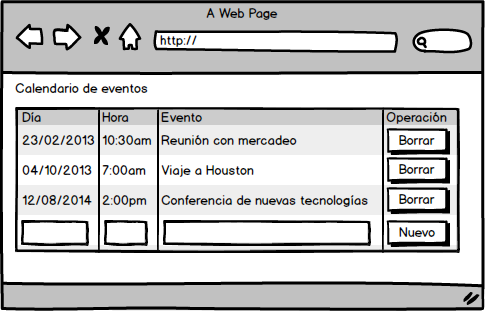
\includegraphics{Eventos.png}
\end{figure}

En este caso se utilizan ``cookies'' para resolver el problema. Note como
se crea un hilera de texto (string) con los diferentes campos a
almacenar utilizando como delimitador el carácter `\textbar{}', y luego se
genera otra hilera de texto con todos los eventos del arreglo pero ahora
delimitados por los caracteres `/n'. Esta última hilera de texto es la
que se almacena en la `cookie'.

\begin{Verbatim}[commandchars=\\\{\}]
\PYGZlt{}?php
  if (isset(\PYGZdl{}\PYGZus{}COOKIE[\PYGZsq{}eventos\PYGZsq{}])) \PYGZob{}
    \PYGZdl{}array = explode(\PYGZdq{}/n\PYGZdq{},\PYGZdl{}\PYGZus{}COOKIE[\PYGZsq{}eventos\PYGZsq{}]);
  \PYGZcb{}  else \PYGZob{}
    \PYGZdl{}array = array();
  \PYGZcb{};

  if (isset(\PYGZdl{}\PYGZus{}POST[\PYGZsq{}borrar\PYGZsq{}])) \PYGZob{}
      \PYGZdl{}id = \PYGZdl{}\PYGZus{}POST[\PYGZsq{}borrar\PYGZsq{}];
      unset(\PYGZdl{}array[\PYGZdl{}id]);
      \PYGZdl{}array = array\PYGZus{}values(\PYGZdl{}array);
      setcookie(\PYGZsq{}eventos\PYGZsq{},implode(\PYGZdq{}/n\PYGZdq{},\PYGZdl{}array));
  \PYGZcb{} else if (isset(\PYGZdl{}\PYGZus{}POST[\PYGZsq{}agregar\PYGZsq{}])) \PYGZob{}
      \PYGZdl{}new\PYGZus{}item = \PYGZdl{}\PYGZus{}POST[\PYGZsq{}dia\PYGZsq{}].\PYGZsq{}\textbar{}\PYGZsq{}.\PYGZdl{}\PYGZus{}POST[\PYGZsq{}hora\PYGZsq{}].\PYGZsq{}\textbar{}\PYGZsq{}.\PYGZdl{}\PYGZus{}POST[\PYGZsq{}evento\PYGZsq{}];
      \PYGZdl{}array[] = \PYGZdl{}new\PYGZus{}item;
      setcookie(\PYGZsq{}eventos\PYGZsq{},implode(\PYGZdq{}/n\PYGZdq{},\PYGZdl{}array));
  \PYGZcb{} else \PYGZob{}
      setcookie(\PYGZsq{}eventos\PYGZsq{},null);
      \PYGZdl{}array = array();
  \PYGZcb{}
?\PYGZgt{}
\PYGZlt{}html\PYGZgt{}
    \PYGZlt{}meta http\PYGZhy{}equiv=\PYGZdq{}Content\PYGZhy{}Type\PYGZdq{} content=\PYGZdq{}text/html; charset=UTF\PYGZhy{}8\PYGZdq{} /\PYGZgt{}
    \PYGZlt{}head\PYGZgt{}
        \PYGZlt{}title\PYGZgt{}Calendario de eventos\PYGZlt{}/title\PYGZgt{}
    \PYGZlt{}/head\PYGZgt{}
    \PYGZlt{}body\PYGZgt{}
      \PYGZlt{}h2\PYGZgt{}Calendario de eventos\PYGZlt{}/h2\PYGZgt{}
      \PYGZlt{}form action=\PYGZdq{}\PYGZlt{}?php echo \PYGZdl{}\PYGZus{}SERVER[\PYGZsq{}PHP\PYGZus{}SELF\PYGZsq{}]; ?\PYGZgt{}\PYGZdq{} method=\PYGZdq{}POST\PYGZdq{}\PYGZgt{}
        \PYGZlt{}table border=1\PYGZgt{}
            \PYGZlt{}tr\PYGZgt{}\PYGZlt{}th\PYGZgt{}Día\PYGZlt{}/th\PYGZgt{}\PYGZlt{}th\PYGZgt{}Hora\PYGZlt{}/th\PYGZgt{}\PYGZlt{}th\PYGZgt{}Evento\PYGZlt{}/th\PYGZgt{}\PYGZlt{}th\PYGZgt{}Operación\PYGZlt{}/th\PYGZgt{}\PYGZlt{}/tr\PYGZgt{}
            \PYGZlt{}?php
              for (\PYGZdl{}i=0;\PYGZdl{}i\PYGZlt{}sizeof(\PYGZdl{}array);\PYGZdl{}i++) \PYGZob{}
                \PYGZdl{}values = explode(\PYGZdq{}\textbar{}\PYGZdq{},\PYGZdl{}array[\PYGZdl{}i]);
                echo \PYGZsq{}\PYGZlt{}tr\PYGZgt{}\PYGZlt{}td\PYGZgt{}\PYGZsq{}.\PYGZdl{}values[0].\PYGZsq{}\PYGZlt{}/td\PYGZgt{}\PYGZlt{}td\PYGZgt{}\PYGZsq{}.\PYGZdl{}values[1].\PYGZsq{}\PYGZlt{}/td\PYGZgt{}\PYGZlt{}td\PYGZgt{}\PYGZsq{}.
                    \PYGZdl{}values[2].\PYGZsq{}\PYGZlt{}/td\PYGZgt{}\PYGZlt{}td\PYGZgt{}\PYGZlt{}button name=\PYGZdq{}borrar\PYGZdq{} value=\PYGZdq{}\PYGZsq{}.\PYGZdl{}i.
                    \PYGZsq{}\PYGZdq{}\PYGZgt{}Borrar\PYGZlt{}/button\PYGZgt{}\PYGZlt{}/td\PYGZgt{}\PYGZlt{}/tr\PYGZgt{}\PYGZsq{};
              \PYGZcb{}
            ?\PYGZgt{}
            \PYGZlt{}tr\PYGZgt{}\PYGZlt{}td\PYGZgt{}\PYGZlt{}input size=\PYGZdq{}10\PYGZdq{} name=\PYGZdq{}dia\PYGZdq{} type=\PYGZdq{}date\PYGZdq{}/\PYGZgt{}\PYGZlt{}/td\PYGZgt{}
                \PYGZlt{}td\PYGZgt{}\PYGZlt{}input name=\PYGZdq{}hora\PYGZdq{} size=\PYGZdq{}10\PYGZdq{} type=\PYGZdq{}time\PYGZdq{}/\PYGZgt{}\PYGZlt{}/td\PYGZgt{}
                \PYGZlt{}td\PYGZgt{}\PYGZlt{}input size=\PYGZdq{}40\PYGZdq{} name=\PYGZdq{}evento\PYGZdq{}/\PYGZgt{}\PYGZlt{}/td\PYGZgt{}
                \PYGZlt{}td\PYGZgt{}\PYGZlt{}button name=\PYGZdq{}agregar\PYGZdq{}\PYGZgt{}Agregar\PYGZlt{}/button\PYGZgt{}\PYGZlt{}/td\PYGZgt{}
            \PYGZlt{}/tr\PYGZgt{}
        \PYGZlt{}/table\PYGZgt{}
      \PYGZlt{}/form\PYGZgt{}
    \PYGZlt{}/body\PYGZgt{}
\PYGZlt{}/html\PYGZgt{}
\end{Verbatim}


\subsection{Ejercicios}
\label{Tutorial3_Sesiones.md:ejercicios}\begin{enumerate}
\item {} 
Intente modificar el ejemplo anterior para manejar los eventos
mediante campos ocultos.

\item {} 
Ahora, intente modificar el mismo ejemplo para almacenar los objetos
mediante variables de sesión.

\end{enumerate}


\section{Manejo de archivos}
\label{Tutorial4_Archivos.md:manejo-de-archivos}\label{Tutorial4_Archivos.md::doc}
La función \emph{fopen(path,mode)} permite abrir un archivo local o mediante
un URL. El \emph{path} del archivo debe incluir la ruta completa al mismo. El
\emph{mode} puede ser \emph{r} - lectura,\emph{w} - escritura,\emph{a} - agregar, o \emph{x}
- escritura exclusiva. Se puede agregar un \emph{+} al modo y si el archivo
no existe, se intentará crear. La función \emph{fclose(file)} cierra un
puntero a un archivo abierto.

La función \emph{feof(file)} comprueba si el puntero a un archivo se
encuentra al final del archivo. La función \emph{fgets(file)} obtiene una
línea desde el puntero a un archivo. La función \emph{file\_exists(file)}
comprueba si existe un archivo o directorio.

\begin{Verbatim}[commandchars=\\\{\}]
\PYGZlt{}?php

\PYGZdl{}path = \PYGZdq{}/home/user/file.txt\PYGZdq{};
if (!file\PYGZus{}exists(\PYGZdl{}path))
    exit(\PYGZdq{}File not found\PYGZdq{});
\PYGZdl{}file = fopen(\PYGZdl{}path, \PYGZdq{}r\PYGZdq{});
if (\PYGZdl{}file) \PYGZob{}
    while ((\PYGZdl{}line = fgets(\PYGZdl{}file)) !== false) \PYGZob{}
        echo \PYGZdl{}line;
    \PYGZcb{}
    if (!feof(\PYGZdl{}file)) \PYGZob{}
        echo \PYGZdq{}Error: EOF not found\PYGZbs{}n\PYGZdq{};
    \PYGZcb{}
    fclose(\PYGZdl{}file);
\PYGZcb{}

?\PYGZgt{}
\end{Verbatim}

La función \emph{fscanf} analiza la entrada desde un archivo de acuerdo a un
formato. Los tipos más importantes son: \emph{\%d} - entero, \emph{\%f} - flotante,
y \emph{\%s} - string. Un detalle importante es que \emph{\%s} no reconoce hileras
de texto con espacios en blanco, únicamente palabras completas.

\begin{Verbatim}[commandchars=\\\{\}]
\PYGZlt{}?php

\PYGZdl{}path = \PYGZdq{}/home/usr/data.txt\PYGZdq{};
if (!file\PYGZus{}exists(\PYGZdl{}path))
    exit(\PYGZdq{}File not found\PYGZdq{});
\PYGZdl{}file = fopen(\PYGZdl{}path, \PYGZdq{}r\PYGZdq{});
echo \PYGZdq{}\PYGZlt{}html\PYGZgt{}\PYGZlt{}body\PYGZgt{}\PYGZlt{}table border=1\PYGZgt{}\PYGZdq{};
echo \PYGZdq{}\PYGZlt{}tr\PYGZgt{}\PYGZlt{}th\PYGZgt{}Country\PYGZlt{}/th\PYGZgt{}\PYGZlt{}th\PYGZgt{}Area\PYGZlt{}/th\PYGZgt{}\PYGZlt{}th\PYGZgt{}Population\PYGZlt{}/th\PYGZgt{}\PYGZlt{}th\PYGZgt{}Density\PYGZlt{}/th\PYGZgt{}\PYGZlt{}/tr\PYGZgt{}\PYGZdq{};
while (\PYGZdl{}data = fscanf(\PYGZdl{}file, \PYGZdq{}\PYGZpc{}s\PYGZbs{}t\PYGZpc{}d\PYGZbs{}t\PYGZpc{}d\PYGZbs{}t\PYGZpc{}f\PYGZbs{}n\PYGZdq{})) \PYGZob{}
    list (\PYGZdl{}country, \PYGZdl{}area, \PYGZdl{}pop, \PYGZdl{}dens) = \PYGZdl{}data;
    echo \PYGZdq{}\PYGZlt{}tr\PYGZgt{}\PYGZlt{}td\PYGZgt{}\PYGZdq{}.\PYGZdl{}country.\PYGZdq{}\PYGZlt{}/td\PYGZgt{}\PYGZlt{}td\PYGZgt{}\PYGZdq{}.\PYGZdl{}area.\PYGZdq{}\PYGZlt{}/td\PYGZgt{}\PYGZlt{}td\PYGZgt{}\PYGZdq{}.
         \PYGZdl{}pop.\PYGZdq{}\PYGZlt{}/td\PYGZgt{}\PYGZlt{}td\PYGZgt{}\PYGZdq{}.\PYGZdl{}dens.\PYGZdq{}\PYGZlt{}/td\PYGZgt{}\PYGZlt{}/tr\PYGZgt{}\PYGZdq{};
\PYGZcb{}
echo \PYGZdq{}\PYGZlt{}/table\PYGZgt{}\PYGZlt{}/body\PYGZgt{}\PYGZlt{}/html\PYGZgt{}\PYGZdq{};
fclose(\PYGZdl{}file);

?\PYGZgt{}
\end{Verbatim}

El archivo de datos para el ejemplo anterior podría ser el siguiente.
Note que debe haber un tabulador que separe cada campo de un mismo
registro.

\begin{Verbatim}[commandchars=\\\{\}]
Belice  22966   334000  14.54
Costa\PYGZus{}Rica  51100   4726000 92.49
El\PYGZus{}Salvador 21041   6108000 290.29
Guatemala   108894  15284000    140.36
Honduras    112492  8447000 75.09
Nicaragua   129494  6028000 46.55
Panama  78200   3652000 46.70
\end{Verbatim}


\subsection{Directorios}
\label{Tutorial4_Archivos.md:directorios}
La función \emph{is\_dir} indica si el nombre del archivo es un directorio y
\emph{is\_file} indica si el nombre de archivo es realmente un archivo. La
función \emph{mkdir} crea un directorio. La función \emph{rename} renombre un
archivo o directorio. La función \emph{rmdir} remueve un directorio y la
función \emph{unlink} remueve un archivo.


\subsection{Archivos binarios}
\label{Tutorial4_Archivos.md:archivos-binarios}
Las funciones \emph{fread} y \emph{fwrite} leen y escriben, respectivamente, en un
archivo en modo binario. La función \emph{fseek} posiciona el puntero del
archivo.

\begin{Verbatim}[commandchars=\\\{\}]
\PYGZlt{}?php

\PYGZdl{}path = \PYGZdq{}/home/usr/data2.txt\PYGZdq{};
if (!file\PYGZus{}exists(\PYGZdl{}path))
    exit(\PYGZdq{}File not found\PYGZdq{});
\PYGZdl{}file = fopen(\PYGZdl{}path, \PYGZdq{}r\PYGZdq{});
echo \PYGZdq{}\PYGZlt{}html\PYGZgt{}\PYGZlt{}body\PYGZgt{}\PYGZlt{}table border=1\PYGZgt{}\PYGZdq{};
echo \PYGZdq{}\PYGZlt{}tr\PYGZgt{}\PYGZlt{}th\PYGZgt{}Country\PYGZlt{}/th\PYGZgt{}\PYGZlt{}th\PYGZgt{}Area\PYGZlt{}/th\PYGZgt{}\PYGZlt{}th\PYGZgt{}Population\PYGZlt{}/th\PYGZgt{}\PYGZlt{}th\PYGZgt{}Density\PYGZlt{}/th\PYGZgt{}\PYGZlt{}/tr\PYGZgt{}\PYGZdq{};
fseek(\PYGZdl{}file,35);
while (\PYGZdl{}data = fread(\PYGZdl{}file, 35)) \PYGZob{}
    \PYGZdl{}fields = explode(\PYGZdq{}\textbar{}\PYGZdq{},\PYGZdl{}data);
    echo \PYGZdq{}\PYGZlt{}tr\PYGZgt{}\PYGZlt{}td\PYGZgt{}\PYGZdq{}.\PYGZdl{}fields[0].\PYGZdq{}\PYGZlt{}/td\PYGZgt{}\PYGZlt{}td\PYGZgt{}\PYGZdq{}.\PYGZdl{}fields[1].\PYGZdq{}\PYGZlt{}/td\PYGZgt{}\PYGZlt{}td\PYGZgt{}\PYGZdq{}.
         \PYGZdl{}fields[2].\PYGZdq{}\PYGZlt{}/td\PYGZgt{}\PYGZlt{}td\PYGZgt{}\PYGZdq{}.\PYGZdl{}fields[3].\PYGZdq{}\PYGZlt{}/td\PYGZgt{}\PYGZlt{}/tr\PYGZgt{}\PYGZdq{};
\PYGZcb{}
echo \PYGZdq{}\PYGZlt{}/table\PYGZgt{}\PYGZlt{}/body\PYGZgt{}\PYGZlt{}/html\PYGZgt{}\PYGZdq{};
fclose(\PYGZdl{}file);

?\PYGZgt{}
\end{Verbatim}

El archivo de datos para el ejemplo anterior podría ser el siguiente.
Note que este es un archivo de registros de tamaño fijo. Además, tome en
cuenta que es necesario omitir los encabezados del archivo.

\begin{Verbatim}[commandchars=\\\{\}]
CountryName\textbar{}Area  \textbar{}People  \textbar{}Densi.
Belice     \textbar{} 22966\textbar{}  334000\textbar{} 14.54
Costa Rica \textbar{} 51100\textbar{} 4726000\textbar{} 92.49
El Salvador\textbar{} 21041\textbar{} 6108000\textbar{}290.29
Guatemala  \textbar{}108894\textbar{}15284000\textbar{}140.36
Honduras   \textbar{}112492\textbar{} 8447000\textbar{} 75.09
Nicaragua  \textbar{}129494\textbar{} 6028000\textbar{} 46.55
Panama     \textbar{} 78200\textbar{} 3652000\textbar{} 46.70
\end{Verbatim}


\subsection{Archivos de texto}
\label{Tutorial4_Archivos.md:archivos-de-texto}
Otra forma de leer archivos de texto es utilizar la función \emph{file}, la
cual transfiere un archivo completo a un arreglo. Note que no es
necesario abrir el archivo (\emph{fopen}) para utilizar este función.

\begin{Verbatim}[commandchars=\\\{\}]
\PYGZlt{}?php

\PYGZdl{}path = \PYGZdq{}/home/usr/data2.txt\PYGZdq{};
if (!file\PYGZus{}exists(\PYGZdl{}path))
    exit(\PYGZdq{}File not found\PYGZdq{});
\PYGZdl{}rows = file(\PYGZdl{}path);
array\PYGZus{}shift(\PYGZdl{}rows);
echo \PYGZdq{}\PYGZlt{}html\PYGZgt{}\PYGZlt{}body\PYGZgt{}\PYGZlt{}table border=1\PYGZgt{}\PYGZdq{};
echo \PYGZdq{}\PYGZlt{}tr\PYGZgt{}\PYGZlt{}th\PYGZgt{}Country\PYGZlt{}/th\PYGZgt{}\PYGZlt{}th\PYGZgt{}Area\PYGZlt{}/th\PYGZgt{}\PYGZlt{}th\PYGZgt{}Population\PYGZlt{}/th\PYGZgt{}\PYGZlt{}th\PYGZgt{}Density\PYGZlt{}/th\PYGZgt{}\PYGZlt{}/tr\PYGZgt{}\PYGZdq{};
foreach (\PYGZdl{}rows as \PYGZdl{}row) \PYGZob{}
    \PYGZdl{}fields = explode(\PYGZdq{}\textbar{}\PYGZdq{},\PYGZdl{}row);
    echo \PYGZdq{}\PYGZlt{}tr\PYGZgt{}\PYGZlt{}td\PYGZgt{}\PYGZdq{}.\PYGZdl{}fields[0].\PYGZdq{}\PYGZlt{}/td\PYGZgt{}\PYGZlt{}td\PYGZgt{}\PYGZdq{}.\PYGZdl{}fields[1].\PYGZdq{}\PYGZlt{}/td\PYGZgt{}\PYGZlt{}td\PYGZgt{}\PYGZdq{}.
         \PYGZdl{}fields[2].\PYGZdq{}\PYGZlt{}/td\PYGZgt{}\PYGZlt{}td\PYGZgt{}\PYGZdq{}.\PYGZdl{}fields[3].\PYGZdq{}\PYGZlt{}/td\PYGZgt{}\PYGZlt{}/tr\PYGZgt{}\PYGZdq{};
\PYGZcb{}
echo \PYGZdq{}\PYGZlt{}/table\PYGZgt{}\PYGZlt{}/body\PYGZgt{}\PYGZlt{}/html\PYGZgt{}\PYGZdq{};

?\PYGZgt{}
\end{Verbatim}


\subsection{Archivos CSV}
\label{Tutorial4_Archivos.md:archivos-csv}
La función \emph{fgetcsv} obtiene una línea del puntero a un archivo y la
examina para tratar campos CSV. La función \emph{fputcsv} da formato a una
línea como CSV y la escribe en un puntero a un archivo.

\begin{Verbatim}[commandchars=\\\{\}]
\PYGZlt{}?php

\PYGZdl{}path = \PYGZdq{}/home/usr/data3.csv\PYGZdq{};
if (!file\PYGZus{}exists(\PYGZdl{}path))
    exit(\PYGZdq{}File not found\PYGZdq{});
\PYGZdl{}file = fopen(\PYGZdl{}path, \PYGZdq{}r\PYGZdq{});
echo \PYGZdq{}\PYGZlt{}html\PYGZgt{}\PYGZlt{}body\PYGZgt{}\PYGZlt{}table border=1\PYGZgt{}\PYGZdq{};
echo \PYGZdq{}\PYGZlt{}tr\PYGZgt{}\PYGZlt{}th\PYGZgt{}Country\PYGZlt{}/th\PYGZgt{}\PYGZlt{}th\PYGZgt{}Area\PYGZlt{}/th\PYGZgt{}\PYGZlt{}th\PYGZgt{}Population\PYGZlt{}/th\PYGZgt{}\PYGZlt{}th\PYGZgt{}Density\PYGZlt{}/th\PYGZgt{}\PYGZlt{}/tr\PYGZgt{}\PYGZdq{};
while (\PYGZdl{}fields = fgetcsv(\PYGZdl{}file,\PYGZdq{},\PYGZdq{})) \PYGZob{}
    echo \PYGZdq{}\PYGZlt{}tr\PYGZgt{}\PYGZlt{}td\PYGZgt{}\PYGZdq{}.\PYGZdl{}fields[0].\PYGZdq{}\PYGZlt{}/td\PYGZgt{}\PYGZlt{}td\PYGZgt{}\PYGZdq{}.\PYGZdl{}fields[1].\PYGZdq{}\PYGZlt{}/td\PYGZgt{}\PYGZlt{}td\PYGZgt{}\PYGZdq{}.
         \PYGZdl{}fields[2].\PYGZdq{}\PYGZlt{}/td\PYGZgt{}\PYGZlt{}td\PYGZgt{}\PYGZdq{}.\PYGZdl{}fields[3].\PYGZdq{}\PYGZlt{}/td\PYGZgt{}\PYGZlt{}/tr\PYGZgt{}\PYGZdq{};
\PYGZcb{}
echo \PYGZdq{}\PYGZlt{}/table\PYGZgt{}\PYGZlt{}/body\PYGZgt{}\PYGZlt{}/html\PYGZgt{}\PYGZdq{};
fclose(\PYGZdl{}file);

?\PYGZgt{}
\end{Verbatim}

El archivo de datos para el ejemplo anterior podría ser el siguiente.

\begin{Verbatim}[commandchars=\\\{\}]
Belice,22966,334000,14.54
Costa Rica,51100,4726000,92.49
El Salvador,21041,6108000,290.29
Guatemala,108894,15284000,140.36
Honduras,112492,8447000,75.09
Nicaragua,129494,6028000,46.55
Panama,78200,3652000,46.70
\end{Verbatim}


\subsection{Ejemplo}
\label{Tutorial4_Archivos.md:ejemplo}
A continuación se muestra un ejemplo de una aplicación Web en PHP que
permite llevar una lista de contactos. Cada contacto tiene un nombre,
teléfono del trabajo, teléfono móvil, dirección electrónica y dirección
postal. Se pueden agregar nuevos contactos, modificar los existentes, o
eliminarlos.
\begin{figure}[htbp]
\centering

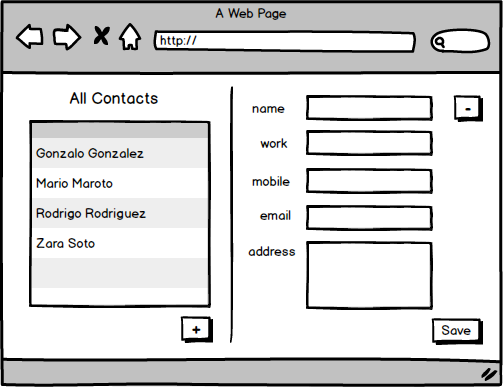
\includegraphics{Agenda.png}
\end{figure}

Note que se utiliza \emph{borrado perezoso} en esta solución, es decir, se
marcan los registros borrados y no se eliminan realmente del archivo.
También, en este ejemplo se utiliza un archivo con registros de tamaño
fijo delimitados por el carácter `\textbar{}'.

\begin{Verbatim}[commandchars=\\\{\}]
\PYGZlt{}?php
\PYGZdl{}path = \PYGZdq{}data.txt\PYGZdq{};
if (file\PYGZus{}exists(\PYGZdl{}path))
  \PYGZdl{}file = fopen(\PYGZdl{}path, \PYGZdq{}r+\PYGZdq{});
else
  \PYGZdl{}file = fopen(\PYGZdl{}path, \PYGZdq{}a+\PYGZdq{});
while (\PYGZdl{}data = fread(\PYGZdl{}file,154)) \PYGZob{}
  \PYGZdl{}array[] = explode(\PYGZsq{}\textbar{}\PYGZsq{},\PYGZdl{}data);
\PYGZcb{};

if (isset(\PYGZdl{}\PYGZus{}GET[\PYGZsq{}get\PYGZsq{}])) \PYGZob{}
  \PYGZdl{}curr = (int)\PYGZdl{}\PYGZus{}GET[\PYGZsq{}get\PYGZsq{}];
  \PYGZdl{}item = \PYGZdl{}array[\PYGZdl{}curr];
\PYGZcb{} else if (isset(\PYGZdl{}\PYGZus{}GET[\PYGZsq{}delete\PYGZsq{}])) \PYGZob{}
  \PYGZdl{}curr = (int)\PYGZdl{}\PYGZus{}GET[\PYGZsq{}delete\PYGZsq{}];
  fseek(\PYGZdl{}file,\PYGZdl{}curr*154,SEEK\PYGZus{}SET);
  fwrite(\PYGZdl{}file,\PYGZsq{}**deleted**\PYGZsq{});
  \PYGZdl{}array[\PYGZdl{}curr][0] = \PYGZsq{}**deleted**\PYGZsq{};
  \PYGZdl{}item = array(\PYGZsq{}\PYGZsq{},\PYGZsq{}\PYGZsq{},\PYGZsq{}\PYGZsq{},\PYGZsq{}\PYGZsq{},\PYGZsq{}\PYGZsq{});
  \PYGZdl{}curr = 0;
\PYGZcb{} else if (isset(\PYGZdl{}\PYGZus{}GET[\PYGZsq{}save\PYGZsq{}])) \PYGZob{}
    \PYGZdl{}curr = (int)\PYGZdl{}\PYGZus{}GET[\PYGZsq{}save\PYGZsq{}];
    \PYGZdl{}item = array(str\PYGZus{}pad(\PYGZdl{}\PYGZus{}GET[\PYGZsq{}name\PYGZsq{}],30),
                  str\PYGZus{}pad(\PYGZdl{}\PYGZus{}GET[\PYGZsq{}work\PYGZsq{}],30),
                  str\PYGZus{}pad(\PYGZdl{}\PYGZus{}GET[\PYGZsq{}mobile\PYGZsq{}],30),
                  str\PYGZus{}pad(\PYGZdl{}\PYGZus{}GET[\PYGZsq{}email\PYGZsq{}],30),
                  str\PYGZus{}pad(\PYGZdl{}\PYGZus{}GET[\PYGZsq{}address\PYGZsq{}],30));
    fseek(\PYGZdl{}file,\PYGZdl{}curr*154,SEEK\PYGZus{}SET);
    fwrite(\PYGZdl{}file,implode(\PYGZsq{}\textbar{}\PYGZsq{},\PYGZdl{}item));
    \PYGZdl{}array[\PYGZdl{}curr] = \PYGZdl{}item;
\PYGZcb{} else if (isset(\PYGZdl{}\PYGZus{}GET[\PYGZsq{}append\PYGZsq{}])) \PYGZob{}
  \PYGZdl{}item = array(\PYGZsq{}\PYGZsq{},\PYGZsq{}\PYGZsq{},\PYGZsq{}\PYGZsq{},\PYGZsq{}\PYGZsq{},\PYGZsq{}\PYGZsq{});
  \PYGZdl{}curr = sizeof(\PYGZdl{}array);
\PYGZcb{};

fclose(\PYGZdl{}file);
?\PYGZgt{}
\PYGZlt{}html\PYGZgt{}
    \PYGZlt{}meta http\PYGZhy{}equiv=\PYGZdq{}Content\PYGZhy{}Type\PYGZdq{} content=\PYGZdq{}text/html; charset=UTF\PYGZhy{}8\PYGZdq{} /\PYGZgt{}
    \PYGZlt{}head\PYGZgt{}
        \PYGZlt{}title\PYGZgt{}Contacts\PYGZlt{}/title\PYGZgt{}
    \PYGZlt{}/head\PYGZgt{}
    \PYGZlt{}body\PYGZgt{}
     \PYGZlt{}form action=\PYGZdq{}\PYGZlt{}?php echo \PYGZdl{}\PYGZus{}SERVER[\PYGZsq{}PHP\PYGZus{}SELF\PYGZsq{}]; ?\PYGZgt{}\PYGZdq{} method=\PYGZdq{}GET\PYGZdq{}\PYGZgt{}
      \PYGZlt{}div style=\PYGZdq{}width: 250px; float: left;\PYGZdq{}\PYGZgt{}
        \PYGZlt{}h3\PYGZgt{}All Contacts\PYGZlt{}/h3\PYGZgt{}
        \PYGZlt{}table width=\PYGZdq{}150\PYGZdq{} border=1\PYGZgt{}
          \PYGZlt{}?php
            for (\PYGZdl{}i=0;\PYGZdl{}i\PYGZlt{}sizeof(\PYGZdl{}array);\PYGZdl{}i++) \PYGZob{}
              if (trim(\PYGZdl{}array[\PYGZdl{}i][0])!=\PYGZdq{}**deleted**\PYGZdq{})
                echo \PYGZsq{}\PYGZlt{}tr\PYGZgt{}\PYGZlt{}td\PYGZgt{}\PYGZlt{}a href=\PYGZdq{}?get=\PYGZsq{}.\PYGZdl{}i.
                     \PYGZsq{}\PYGZdq{} style=\PYGZdq{}text\PYGZhy{}decoration:none;\PYGZdq{}\PYGZgt{}\PYGZsq{}.
                     \PYGZdl{}array[\PYGZdl{}i][0].\PYGZsq{}\PYGZlt{}/a\PYGZgt{}\PYGZlt{}/td\PYGZgt{}\PYGZlt{}/tr\PYGZgt{}\PYGZsq{};
            \PYGZcb{}
          ?\PYGZgt{}
        \PYGZlt{}/table\PYGZgt{}
        \PYGZlt{}/p\PYGZgt{}
        \PYGZlt{}button name=\PYGZdq{}append\PYGZdq{} value=\PYGZdq{}\PYGZdq{}\PYGZgt{}+\PYGZlt{}/button\PYGZgt{}
      \PYGZlt{}/div\PYGZgt{}
      \PYGZlt{}div style=\PYGZdq{}margin\PYGZhy{}left:250px;\PYGZdq{}\PYGZgt{}
          \PYGZlt{}table\PYGZgt{}
            \PYGZlt{}tr\PYGZgt{}\PYGZlt{}td\PYGZgt{}\PYGZam{}nbsp;\PYGZlt{}/td\PYGZgt{}\PYGZlt{}/tr\PYGZgt{}
            \PYGZlt{}tr\PYGZgt{}\PYGZlt{}td\PYGZgt{}\PYGZlt{}label\PYGZgt{}name\PYGZlt{}/label\PYGZgt{}\PYGZlt{}/td\PYGZgt{}\PYGZlt{}td\PYGZgt{}
                \PYGZlt{}input name=\PYGZdq{}name\PYGZdq{} size=\PYGZdq{}30\PYGZdq{} value=\PYGZdq{}\PYGZlt{}?php echo \PYGZdl{}item[0]; ?\PYGZgt{}\PYGZdq{}/\PYGZgt{}\PYGZlt{}/td\PYGZgt{}\PYGZlt{}/tr\PYGZgt{}
            \PYGZlt{}tr\PYGZgt{}\PYGZlt{}td\PYGZgt{}\PYGZlt{}label\PYGZgt{}work\PYGZlt{}/label\PYGZgt{}\PYGZlt{}/td\PYGZgt{}\PYGZlt{}td\PYGZgt{}
                \PYGZlt{}input name=\PYGZdq{}work\PYGZdq{} size=\PYGZdq{}30\PYGZdq{} value=\PYGZdq{}\PYGZlt{}?php echo \PYGZdl{}item[1]; ?\PYGZgt{}\PYGZdq{}/\PYGZgt{}\PYGZlt{}/td\PYGZgt{}\PYGZlt{}/tr\PYGZgt{}
            \PYGZlt{}tr\PYGZgt{}\PYGZlt{}td\PYGZgt{}\PYGZlt{}label\PYGZgt{}mobile\PYGZlt{}/label\PYGZgt{}\PYGZlt{}/td\PYGZgt{}\PYGZlt{}td\PYGZgt{}
                \PYGZlt{}input name=\PYGZdq{}mobile\PYGZdq{} size=\PYGZdq{}30\PYGZdq{} value=\PYGZdq{}\PYGZlt{}?php echo \PYGZdl{}item[2]; ?\PYGZgt{}\PYGZdq{}/\PYGZgt{}\PYGZlt{}/td\PYGZgt{}\PYGZlt{}/tr\PYGZgt{}
            \PYGZlt{}tr\PYGZgt{}\PYGZlt{}td\PYGZgt{}\PYGZlt{}label\PYGZgt{}email\PYGZlt{}/label\PYGZgt{}\PYGZlt{}/td\PYGZgt{}\PYGZlt{}td\PYGZgt{}
                \PYGZlt{}input name=\PYGZdq{}email\PYGZdq{} size=\PYGZdq{}30\PYGZdq{} value=\PYGZdq{}\PYGZlt{}?php echo \PYGZdl{}item[3]; ?\PYGZgt{}\PYGZdq{}/\PYGZgt{}\PYGZlt{}/td\PYGZgt{}\PYGZlt{}/tr\PYGZgt{}
            \PYGZlt{}tr\PYGZgt{}\PYGZlt{}td\PYGZgt{}\PYGZlt{}label\PYGZgt{}address\PYGZlt{}/label\PYGZgt{}\PYGZlt{}/td\PYGZgt{}\PYGZlt{}td\PYGZgt{}
                \PYGZlt{}input name=\PYGZdq{}address\PYGZdq{} size=\PYGZdq{}30\PYGZdq{} value=\PYGZdq{}\PYGZlt{}?php echo \PYGZdl{}item[4]; ?\PYGZgt{}\PYGZdq{}/\PYGZgt{}\PYGZlt{}/td\PYGZgt{}\PYGZlt{}/tr\PYGZgt{}
            \PYGZlt{}tr\PYGZgt{}\PYGZlt{}td\PYGZgt{}\PYGZam{}nbsp;\PYGZlt{}/td\PYGZgt{}\PYGZlt{}/tr\PYGZgt{}
            \PYGZlt{}tr\PYGZgt{}\PYGZlt{}td\PYGZgt{}\PYGZlt{}button name=\PYGZdq{}delete\PYGZdq{} value=\PYGZdq{}\PYGZlt{}?php echo \PYGZdl{}curr; ?\PYGZgt{}\PYGZdq{}\PYGZgt{}\PYGZhy{}\PYGZlt{}/button\PYGZgt{}\PYGZlt{}/td\PYGZgt{}
                \PYGZlt{}td align=\PYGZdq{}right\PYGZdq{}\PYGZgt{}
                \PYGZlt{}button name=\PYGZdq{}save\PYGZdq{} value=\PYGZdq{}\PYGZlt{}?php echo \PYGZdl{}curr; ?\PYGZgt{}\PYGZdq{}\PYGZgt{}Save\PYGZlt{}/button\PYGZgt{}\PYGZlt{}/td\PYGZgt{}\PYGZlt{}/tr\PYGZgt{}
          \PYGZlt{}/table\PYGZgt{}
        \PYGZlt{}/div\PYGZgt{}
      \PYGZlt{}/form\PYGZgt{}
    \PYGZlt{}/body\PYGZgt{}
\PYGZlt{}/html\PYGZgt{}
\end{Verbatim}


\subsection{Ejercicios}
\label{Tutorial4_Archivos.md:ejercicios}\begin{enumerate}
\item {} 
Intente modificar el ejemplo anterior para que utilice dos archivos,
uno que almacene el nombre del contacto y un índice. Este índice
indicará la posición en otro archivo en donde se encontrará el
detalle del contacto.

\item {} 
Ahora, intente modificar el ejemplo para resolver el mismo problema
pero utilizando registros de tamaño variable. Trate de solucionar de
una forma `elegante' el borrado de registros.

\item {} 
Debido a que cada vez que se ejecuta la aplicación es necesario
cargar todo el archivo en memoria, una mejor solución sería `paginar'
los registros, es decir, cargar solo una pequeña parte en memoria y
permitir que el usuario cargara más registros conforme los necesite
(posiblemente mediante un par de botones adicionales).

\end{enumerate}


\section{Bases de datos con PDO}
\label{Tutorial5_BasesDatos.md::doc}\label{Tutorial5_BasesDatos.md:bases-de-datos-con-pdo}
La extensión PDO (PHP Data Objects) de PHP consiste de una capa de
abstracción para acceder a diferentes tipos de bases de datos.
Utilizando PDO se logran estandarizar los diferentes mecanismos para
realizar la conexión a una base de datos, así como recuperar y modificar
información. Sin embargo, PDO no estandariza SQL lo que significa que se
debe lidiar con las diferentes sintaxis de las instrucciones en cada
administrador de bases de datos.


\subsection{Manejadores de bases de datos}
\label{Tutorial5_BasesDatos.md:manejadores-de-bases-de-datos}
Para cada base de datos existe un manejador (driver) específico, que
debe estar habilitado en el archivo de configuración de PHP (el archivo
\emph{php.ini}). Los manejadores se administran mediante extensiones de PHP,
las cuales tienen nombres finalizando con \emph{dll} en Windows y con \emph{so} en
Unix.

\begin{Verbatim}[commandchars=\\\{\}]
\PYG{n}{extension}\PYG{o}{=}\PYG{n}{php\PYGZus{}pdo}\PYG{o}{.}\PYG{n}{dll}
\PYG{n}{extension}\PYG{o}{=}\PYG{n}{php\PYGZus{}pdo\PYGZus{}firebird}\PYG{o}{.}\PYG{n}{dll}
\PYG{n}{extension}\PYG{o}{=}\PYG{n}{php\PYGZus{}pdo\PYGZus{}informix}\PYG{o}{.}\PYG{n}{dll}
\PYG{n}{extension}\PYG{o}{=}\PYG{n}{php\PYGZus{}pdo\PYGZus{}mssql}\PYG{o}{.}\PYG{n}{dll}
\PYG{n}{extension}\PYG{o}{=}\PYG{n}{php\PYGZus{}pdo\PYGZus{}mysql}\PYG{o}{.}\PYG{n}{dll}
\PYG{n}{extension}\PYG{o}{=}\PYG{n}{php\PYGZus{}pdo\PYGZus{}oci}\PYG{o}{.}\PYG{n}{dll}
\PYG{n}{extension}\PYG{o}{=}\PYG{n}{php\PYGZus{}pdo\PYGZus{}oci8}\PYG{o}{.}\PYG{n}{dll}
\PYG{n}{extension}\PYG{o}{=}\PYG{n}{php\PYGZus{}pdo\PYGZus{}odbc}\PYG{o}{.}\PYG{n}{dll}
\PYG{n}{extension}\PYG{o}{=}\PYG{n}{php\PYGZus{}pdo\PYGZus{}pgsql}\PYG{o}{.}\PYG{n}{dll}
\PYG{n}{extension}\PYG{o}{=}\PYG{n}{php\PYGZus{}pdo\PYGZus{}sqlite}\PYG{o}{.}\PYG{n}{dll}
\end{Verbatim}

Todas estas extensiones deben existir en el directorio de \emph{extensiones}
de PHP. Generalmente las extensiones \emph{php\_pdo} y \emph{php\_pdo\_sqlite}
estarán habilitadas por omisión.


\subsection{Conexiones}
\label{Tutorial5_BasesDatos.md:conexiones}
Para realizar una nueva conexión se debe crear una instancia del objeto
\emph{PDO}. Este constructor acepta una serie de parámetros de conexión
(string de conexión) que pueden ser específicos para cada sistema de
bases de datos.

Si no se logra establecer la conexión se producirá una excepción
(PDOException). Si la conexión es exitosa, una instancia de \emph{PDO} será
devuelta. La conexión permanece activa por todo le ciclo de vida del
objeto \emph{PDO}. Para cerrar la conexión, se debe destruir el objeto
asegurándose que toda referencia sea eliminada, o bien, PHP cerrará la
conexión automáticamente cuando el programa finalice.

Si se desea hacer una conexión persistente, que no sea eliminada al
final de la ejecución del programa, es necesario habilitar la opción
\emph{PDO:ATTR\_PERSISTENT} en el arreglo de las opciones de la conexión.

\begin{Verbatim}[commandchars=\\\{\}]
\PYGZlt{}?php
try \PYGZob{}
    \PYGZdl{}dbh = new PDO(\PYGZsq{}sqlite:test.db\PYGZsq{});
    \PYGZdl{}dbh\PYGZhy{}\PYGZgt{}exec(\PYGZdq{}CREATE TABLE countries
                 (name TEXT, area INTEGER, population INTEGER, density REAL)\PYGZdq{});
    \PYGZdl{}dbh = null;
\PYGZcb{} catch (PDOException \PYGZdl{}e) \PYGZob{}
    print \PYGZdq{}Error!: \PYGZdq{} . \PYGZdl{}e\PYGZhy{}\PYGZgt{}getMessage() . \PYGZdq{}\PYGZlt{}br/\PYGZgt{}\PYGZdq{};
    die();
\PYGZcb{}
?\PYGZgt{}
\end{Verbatim}

Note que en el ejemplo anterior la base de datos podría ser creada
usando el comando \emph{sqlite3 test.db ``''} (si está disponible en el
ambiente). Además, el archivo \emph{test.db} como el directorio en que se
encuentra, deben tener derechos de escritura.


\subsection{Transacciones}
\label{Tutorial5_BasesDatos.md:transacciones}
Debido a que no todas las bases de datos soportan transacciones, PHP
corre en el modo de \emph{auto-commit} que ejecuta cada instrucción
individual en forma implícita. Si se desea usar transacciones, y no se
desea utilizar el modo de \emph{auto-commit}, es necesario invocar el método
\emph{PDO::beginTransaction()} al inicio de la transacción. Si el manejador
de la base de datos no permite el uso de transacciones se producirá una
excepción (\emph{PDOException}). Cuando se acabe de especificar la
transacción se pueden utilizar los métodos \emph{PDO::Commit} para aplicar
dichas instrucciones, o bien, \emph{PDO::rollBack} para abortar dicha
transacción.

\begin{Verbatim}[commandchars=\\\{\}]
\PYGZlt{}?php
try \PYGZob{}
  \PYGZdl{}dbh = new PDO(\PYGZsq{}sqlite:test.db\PYGZsq{});
  echo \PYGZdq{}Connected\PYGZbs{}n\PYGZdq{};
\PYGZcb{} catch (Exception \PYGZdl{}e) \PYGZob{}
  die(\PYGZdq{}Unable to connect: \PYGZdq{} . \PYGZdl{}e\PYGZhy{}\PYGZgt{}getMessage());
\PYGZcb{}

try \PYGZob{}

  \PYGZdl{}dbh\PYGZhy{}\PYGZgt{}beginTransaction();
  \PYGZdl{}dbh\PYGZhy{}\PYGZgt{}exec(\PYGZdq{}INSERT INTO countries (name, area, population, density)
                          values (\PYGZsq{}Belice\PYGZsq{},22966,334000,14.54)\PYGZdq{});
  \PYGZdl{}dbh\PYGZhy{}\PYGZgt{}exec(\PYGZdq{}INSERT INTO countries (name, area, population, density)
                          values (\PYGZsq{}Costa Rica\PYGZsq{},51100,4726000,92.49)\PYGZdq{});
  \PYGZdl{}dbh\PYGZhy{}\PYGZgt{}exec(\PYGZdq{}INSERT INTO countries (name, area, population, density)
                          values (\PYGZsq{}El Salvador\PYGZsq{},21041,6108000,290.29)\PYGZdq{});
  \PYGZdl{}dbh\PYGZhy{}\PYGZgt{}exec(\PYGZdq{}INSERT INTO countries (name, area, population, density)
                          values (\PYGZsq{}Guatemala\PYGZsq{},108894,15284000,140.36)\PYGZdq{});
  \PYGZdl{}dbh\PYGZhy{}\PYGZgt{}exec(\PYGZdq{}INSERT INTO countries (name, area, population, density)
                          values (\PYGZsq{}Honduras\PYGZsq{},112492,8447000,75.09)\PYGZdq{});
  \PYGZdl{}dbh\PYGZhy{}\PYGZgt{}commit();

\PYGZcb{} catch (Exception \PYGZdl{}e) \PYGZob{}
  \PYGZdl{}dbh\PYGZhy{}\PYGZgt{}rollBack();
  echo \PYGZdq{}Failed: \PYGZdq{} . \PYGZdl{}e\PYGZhy{}\PYGZgt{}getMessage();
\PYGZcb{}
?\PYGZgt{}
\end{Verbatim}

Si una transacción no fue terminada con la instrucción \emph{commit} y el
programa finaliza, la base de datos abortará la transacción
automáticamente.


\subsection{Instrucciones preparadas}
\label{Tutorial5_BasesDatos.md:instrucciones-preparadas}
Una \emph{instrucción preparada} es un tipo de plantilla para SQL que puede
ser personalizada utilizando parámetros. Existen dos beneficios de
utilizar \emph{instrucciones preparadas} : la base de datos únicamente
compilará una vez la instrucción lo cual ahorra mucho tiempo, y los
parámetros no necesitan \emph{comillas} ya que el manejador se encarga de
agregarlas a la instrucción. El realizar el enlace (bind) de parámetros
se puede realizar por mediante el nombre del parámetro o por posición
(utilizando el símbolo ?).

\begin{Verbatim}[commandchars=\\\{\}]
\PYGZlt{}?php
try \PYGZob{}
  \PYGZdl{}dbh = new PDO(\PYGZsq{}sqlite:test.db\PYGZsq{});
  echo \PYGZdq{}Connected\PYGZbs{}n\PYGZdq{};
\PYGZcb{} catch (Exception \PYGZdl{}e) \PYGZob{}
  die(\PYGZdq{}Unable to connect: \PYGZdq{} . \PYGZdl{}e\PYGZhy{}\PYGZgt{}getMessage());
\PYGZcb{}

try \PYGZob{}
  \PYGZdl{}stmt = \PYGZdl{}dbh\PYGZhy{}\PYGZgt{}prepare(\PYGZdq{}INSERT INTO countries (name, area, population, density)
                                VALUES (:name, :area, :population, :density)\PYGZdq{});
  \PYGZdl{}stmt\PYGZhy{}\PYGZgt{}bindParam(\PYGZsq{}:name\PYGZsq{}, \PYGZdl{}name);
  \PYGZdl{}stmt\PYGZhy{}\PYGZgt{}bindParam(\PYGZsq{}:area\PYGZsq{}, \PYGZdl{}area);
  \PYGZdl{}stmt\PYGZhy{}\PYGZgt{}bindParam(\PYGZsq{}:population\PYGZsq{}, \PYGZdl{}population);
  \PYGZdl{}stmt\PYGZhy{}\PYGZgt{}bindParam(\PYGZsq{}:density\PYGZsq{}, \PYGZdl{}density);

  \PYGZdl{}dbh\PYGZhy{}\PYGZgt{}beginTransaction();
  \PYGZdl{}name = \PYGZsq{}Nicaragua\PYGZsq{}; \PYGZdl{}area = 129494; \PYGZdl{}population = 602800; \PYGZdl{}density = 46.55;
  \PYGZdl{}stmt\PYGZhy{}\PYGZgt{}execute();
  \PYGZdl{}name = \PYGZsq{}Panama\PYGZsq{}; \PYGZdl{}area = 78200; \PYGZdl{}population = 3652000; \PYGZdl{}density = 46.70;
  \PYGZdl{}stmt\PYGZhy{}\PYGZgt{}execute();
  \PYGZdl{}dbh\PYGZhy{}\PYGZgt{}commit();

\PYGZcb{} catch (Exception \PYGZdl{}e) \PYGZob{}
  \PYGZdl{}dbh\PYGZhy{}\PYGZgt{}rollBack();
  echo \PYGZdq{}Failed: \PYGZdq{} . \PYGZdl{}e\PYGZhy{}\PYGZgt{}getMessage();
\PYGZcb{}
?\PYGZgt{}
\end{Verbatim}

Adicionalmente, es posible utilizar un arreglo para pasar los parámetros
de la consulta. En este caso no es necesario incluir el enlace (bind) de
parámetros. Es importante notar que el orden de los parámetros resulta
vital aquí.

\begin{Verbatim}[commandchars=\\\{\}]
\PYGZlt{}?php
try \PYGZob{}
  \PYGZdl{}dbh = new PDO(\PYGZsq{}sqlite:test.db\PYGZsq{});
  echo \PYGZdq{}Connected\PYGZbs{}n\PYGZdq{};
\PYGZcb{} catch (Exception \PYGZdl{}e) \PYGZob{}
  die(\PYGZdq{}Unable to connect: \PYGZdq{} . \PYGZdl{}e\PYGZhy{}\PYGZgt{}getMessage());
\PYGZcb{}

try \PYGZob{}
  \PYGZdl{}stmt = \PYGZdl{}dbh\PYGZhy{}\PYGZgt{}prepare(\PYGZdq{}INSERT INTO countries (name, area, population, density)
                                VALUES (?, ?, ?, ?)\PYGZdq{});

  \PYGZdl{}dbh\PYGZhy{}\PYGZgt{}beginTransaction();
  \PYGZdl{}stmt\PYGZhy{}\PYGZgt{}execute(array(\PYGZsq{}Nicaragua\PYGZsq{}, 129494, 602800, 46.55));
  \PYGZdl{}stmt\PYGZhy{}\PYGZgt{}execute(array(\PYGZsq{}Panama\PYGZsq{}, 78200, 3652000, 46.70));
  \PYGZdl{}dbh\PYGZhy{}\PYGZgt{}commit();

\PYGZcb{} catch (Exception \PYGZdl{}e) \PYGZob{}
  \PYGZdl{}dbh\PYGZhy{}\PYGZgt{}rollBack();
  echo \PYGZdq{}Failed: \PYGZdq{} . \PYGZdl{}e\PYGZhy{}\PYGZgt{}getMessage();
\PYGZcb{}
?\PYGZgt{}
\end{Verbatim}


\subsection{Recuperación de datos}
\label{Tutorial5_BasesDatos.md:recuperacion-de-datos}
El método \emph{PDOStatement::fetch} permite obtener la siguiente fila de un
conjunto de resultados de una consulta. Esta instrucción tiene varios
estilos de recuperación,entre ellos:
\begin{itemize}
\item {} 
PDO::FETCH\_NUM: Retorna la siguiente fila como un arreglo indexado
por posición.

\item {} 
PDO::FETCH\_ASSOC: Retorna la siguiente fila como un arreglo indexado
por el nombre de la columna.

\item {} 
PDO::FETCH\_OBJ: Retorna la siguiente fila como un objeto anónimo con
los nombres de las columnas como propiedades.

\end{itemize}

Si se produce un error, la instrucción \emph{fetch} retornará \emph{FALSE}.

\begin{Verbatim}[commandchars=\\\{\}]
\PYGZlt{}html\PYGZgt{}
\PYGZlt{}?php
try \PYGZob{}
  \PYGZdl{}dbh = new PDO(\PYGZsq{}sqlite:test.db\PYGZsq{});
\PYGZcb{} catch (Exception \PYGZdl{}e) \PYGZob{}
  die(\PYGZdq{}Unable to connect: \PYGZdq{} . \PYGZdl{}e\PYGZhy{}\PYGZgt{}getMessage());
\PYGZcb{}
try \PYGZob{}
    \PYGZdl{}sth = \PYGZdl{}dbh\PYGZhy{}\PYGZgt{}prepare(\PYGZdq{}SELECT * FROM countries\PYGZdq{});
    \PYGZdl{}sth\PYGZhy{}\PYGZgt{}execute();
    echo \PYGZdq{}\PYGZlt{}table border=1\PYGZgt{}\PYGZdq{};
    echo \PYGZdq{}\PYGZlt{}tr\PYGZgt{}\PYGZlt{}th\PYGZgt{}Country\PYGZlt{}/th\PYGZgt{}\PYGZlt{}th\PYGZgt{}Area\PYGZlt{}/th\PYGZgt{}\PYGZlt{}th\PYGZgt{}People\PYGZlt{}/th\PYGZgt{}\PYGZlt{}th\PYGZgt{}Dens.\PYGZlt{}/th\PYGZgt{}\PYGZlt{}/tr\PYGZgt{}\PYGZdq{};
    while (\PYGZdl{}result = \PYGZdl{}sth\PYGZhy{}\PYGZgt{}fetch(PDO::FETCH\PYGZus{}ASSOC)) \PYGZob{}
        echo \PYGZdq{}\PYGZlt{}tr\PYGZgt{}\PYGZlt{}td\PYGZgt{}\PYGZdq{}.\PYGZdl{}result[\PYGZsq{}name\PYGZsq{}].\PYGZdq{}\PYGZlt{}/td\PYGZgt{}\PYGZlt{}td\PYGZgt{}\PYGZdq{}.\PYGZdl{}result[\PYGZsq{}area\PYGZsq{}].
            \PYGZdq{}\PYGZlt{}/td\PYGZgt{}\PYGZlt{}td\PYGZgt{}\PYGZdq{}.\PYGZdl{}result[\PYGZsq{}population\PYGZsq{}].\PYGZdq{}\PYGZlt{}/td\PYGZgt{}\PYGZlt{}td\PYGZgt{}\PYGZdq{}.\PYGZdl{}result[\PYGZsq{}density\PYGZsq{}].
            \PYGZdq{}\PYGZlt{}/td\PYGZgt{}\PYGZlt{}/tr\PYGZgt{}\PYGZdq{};
    \PYGZcb{}
    echo \PYGZdq{}\PYGZlt{}/table\PYGZgt{}\PYGZdq{};
\PYGZcb{} catch (Exception \PYGZdl{}e) \PYGZob{}
  echo \PYGZdq{}Failed: \PYGZdq{} . \PYGZdl{}e\PYGZhy{}\PYGZgt{}getMessage();
\PYGZcb{}
?\PYGZgt{}
\PYGZlt{}/html\PYGZgt{}
\end{Verbatim}

Por su parte la instrucción \emph{PDOStatement::fetchAll} retornará un
arreglo conteniendo todos las filas de un conjunto de resultados. El
arreglo representa cada columna como un arreglo de valores por columnas
o un objeto en donde las propiedades corresponden a los nombres de las
columnas. Esta instrucción cuenta con varios modos al igual que la
instrucción \emph{fetch}, e inclusive se pueden especificar las columnas que
se desean recuperar. Se retorna un arreglo vacío si no existen
resultados, o \emph{FALSE} si la consulta falla.

El siguiente ejemplo muestra el uso de la instrucción \emph{fetchAll} , y al
mismo tiempo se muestra una forma de recuperar los datos cuando no se
conocen de antemano los nombres de las columnas ni la cantidad de ellas.

\begin{Verbatim}[commandchars=\\\{\}]
\PYGZlt{}html\PYGZgt{}
    \PYGZlt{}?php
    try \PYGZob{}
      \PYGZdl{}dbh = new PDO(\PYGZsq{}sqlite:test.db\PYGZsq{});
    \PYGZcb{} catch (Exception \PYGZdl{}e) \PYGZob{}
      die(\PYGZdq{}Unable to connect: \PYGZdq{} . \PYGZdl{}e\PYGZhy{}\PYGZgt{}getMessage());
    \PYGZcb{}

    try \PYGZob{}
        \PYGZdl{}sth = \PYGZdl{}dbh\PYGZhy{}\PYGZgt{}prepare(\PYGZdq{}SELECT * FROM countries\PYGZdq{});
        \PYGZdl{}sth\PYGZhy{}\PYGZgt{}execute();
        echo \PYGZdq{}\PYGZlt{}table border=1\PYGZgt{}\PYGZlt{}tr\PYGZgt{}\PYGZdq{};
        \PYGZdl{}result = \PYGZdl{}sth\PYGZhy{}\PYGZgt{}fetchAll(PDO::FETCH\PYGZus{}ASSOC);
        \PYGZdl{}keys = array\PYGZus{}keys(\PYGZdl{}result[0]);
        foreach (\PYGZdl{}keys as \PYGZdl{}key)
          echo \PYGZdq{}\PYGZlt{}th\PYGZgt{}\PYGZdq{}.\PYGZdl{}key.\PYGZdq{}\PYGZlt{}/th\PYGZgt{}\PYGZdq{};
        echo \PYGZdq{}\PYGZlt{}/tr\PYGZgt{}\PYGZdq{};
        foreach (\PYGZdl{}result as \PYGZdl{}row) \PYGZob{}
          echo \PYGZdq{}\PYGZlt{}tr\PYGZgt{}\PYGZdq{};
          foreach (\PYGZdl{}keys as \PYGZdl{}key)
              echo \PYGZdq{}\PYGZlt{}td\PYGZgt{}\PYGZdq{}.\PYGZdl{}row[\PYGZdl{}key].\PYGZdq{}\PYGZlt{}/td\PYGZgt{}\PYGZdq{};
          echo \PYGZdq{}\PYGZlt{}/tr\PYGZgt{}\PYGZdq{};
        \PYGZcb{}
        echo \PYGZdq{}\PYGZlt{}/table\PYGZgt{}\PYGZdq{};
    \PYGZcb{} catch (Exception \PYGZdl{}e) \PYGZob{}
      echo \PYGZdq{}Failed: \PYGZdq{} . \PYGZdl{}e\PYGZhy{}\PYGZgt{}getMessage();
    \PYGZcb{}
    ?\PYGZgt{}
\PYGZlt{}/html\PYGZgt{}
\end{Verbatim}



\renewcommand{\indexname}{Índice}
\printindex
\end{document}
